% \documentclass[11pt]{article}
\documentclass[review]{elsarticle}

\usepackage{lineno,hyperref}
\modulolinenumbers[5]
\linenumbers
\journal{Egyptian Informatics Journal}
% -----------------------------
% Packages (minimal, common)
% -----------------------------
\usepackage[a4paper,margin=1in]{geometry}
\usepackage{microtype}
\usepackage{hyperref}
\usepackage{enumitem}
\usepackage{graphicx}
\usepackage{booktabs}
\usepackage{amsmath,amssymb}
\usepackage{tikz}
\usetikzlibrary{shapes.geometric, shapes.symbols, arrows.meta, positioning, fit, backgrounds, calc}
\usepackage{float}
\usepackage{todonotes}
\usepackage{tabularx}
\usepackage{multirow}
% -----------------------------
% Metadata
% -----------------------------

% \author{, Ahmed Awad}
% \date{\today}

\begin{document}
\begin{frontmatter}
    % \title{STREAMTRACK: Multi-Camera Object Tracking Using Streams and Tables}
    \title{STREAMTRACK: A Streams-and-Tables Architecture for Scalable and Reconfigurable Multi-Camera Object Tracking}
    \author[add1]{Mahmoud Tayee}%\email{23001546@ug.buid.ac.ae}
    \ead{m.mostafa2118@nu.edu.eg}
    \author[add1]{Mohamed ElHelw}%\email{23001546@ug.buid.ac.ae}
    \ead{melhelw@nu.edu.eg}
    \author[add2,add3]{Ahmed Awad\corref{mycorrespondingauthor}}
    \cortext[mycorrespondingauthor]{Corresponding author}
    \ead{a.gaafar@fci-cu.edu.eg}

\address[add1]{Nile University, Giza, Egypt}
\address[add2]{Faculty of Computers and Artificial Intelligence, Cairo University, Egypt}
\address[add3]{The British University in Dubai, Dubai, The UAE}

\begin{abstract}
Multi-camera object tracking (MCOT) is typically built as a tightly coupled, monolithic computer-vision pipeline, which makes cross-camera association hard to scale, identity decisions hard to inspect, and the camera network hard to reconfigure. We argue these are problems of \emph{architecture}, not of the vision task, and re-architect MCOT as a \emph{streams-and-tables} system: detections flow as streams, global identities and camera topology are queryable relational tables, and cross-camera association is a continuous, topology-aware join over them. 
This turns each difficulty into a property of the design: topology-pruned association (scalability), an inspectable identity view (observability), and topology-as-data (zero-downtime reconfigurability). Realised on an embeddable complex-event-processing engine, the architecture reproduces the
global-identity assignments of a state-of-the-art batch baseline while delivering a \textbf{9.8$\times$} overall speedup (up to \textbf{300$\times$} in representative selection and \textbf{236$\times$} in clustering) over an equivalent JVM-native batch implementation, isolating the architectural speedup from language, runtime, and library effects, with a further \textbf{4.16$\times$} latency reduction (\textbf{4.27$\times$} in
steady state) from topology-aware partitioning at nine cameras.

\end{abstract}


\begin{keyword}
Stream Processing\sep Complex Event Processing\sep Software Architecture\sep Multi-camera Object Tracking\sep Streams and Tables\sep Edge Computing
\end{keyword}

\end{frontmatter}
% \maketitle


\section{Introduction}
\label{sec:intro}

Multi-camera object tracking (MCOT) underpins a growing class of applications, such as urban traffic management~\cite{9151096} and public-space surveillance~\cite{thirde2006multi,bhuyan2007tracking} .%\todo{student[Done]: cite 2--3 representative MCOT application papers}. 
The task is to assign a single,
consistent global identity to each physical object as it moves across a network of cameras. Such systems must meet not only computer-vision accuracy targets but also operational
demands, scaling to more cameras, exposing intermediate decisions for debugging, and adapting to changes in the camera network topology.

These operational demands are where conventional MCOT systems struggle. We argue the cause is \emph{architectural} rather than algorithmic. Such systems are typically built as tightly coupled,
monolithic computer-vision pipelines in which cross-camera association logic, identity state, and
network topology are entangled in bespoke imperative code~\cite{yoshida2024overlap,kim2024cluster,xie2024robust} %\todo{student[Done]: cite representative monolithic/MTMC pipelines, e.g. AI City Challenge entries}
. This coupling is precisely what makes association hard to scale (matching defaults to all camera pairs), state hard to inspect (identity decisions live in in-memory program variables), and camera network topology hard to change (re-linking cameras means editing code and restarting the pipeline, losing accumulated state). Treating these as vision problems misdiagnoses them; they are consequences of the system's architecture.

We address them by re-architecting MCOT as a \emph{streams-and-tables} system. Per-camera detections and tracklet updates flow as append-only \emph{streams}; global identities and the
camera-network topology are maintained as mutable, queryable relational \emph{tables}; and cross-camera association is expressed as continuous CQL queries over them, realised as
topology-aware stream joins parametrised by a live camera-neighbourhood table. This rests on the
stream--table duality from data-stream management~\cite{sax2018streams,DBLP:conf/dbpl/ArasuBW03},
and is not specific to vision: we previously showed that the same paradigm transforms a stream engine into a process-orchestration engine~\cite{awad2025best}. Demonstrating it now on a problem
as different as multi-camera perception is evidence that streams-and-tables is a general architectural approach for re-engineering monolithic, stateful reactive systems pipelines, not a one-off technique.

The reframing is valuable because it turns each operational difficulty into a property obtained by construction. Pruning association to topological neighbourhoods makes it \emph{scalable}; maintaining identity in a relational table makes the system's state \emph{inspectable}; and representing topology
as data makes the network \emph{reconfigurable at runtime}, \emph{without any code changes or pipeline restarts}.
We realise the architecture on Esper, an embeddable complex-event-processing engine, in a single process where high-dimensional appearance tensors are referenced by object identity and shared
in memory without serialisation.

This paper makes the following contributions:
\begin{itemize}[leftmargin=*]
    \item \textbf{A streams-and-tables re-architecting of MCOT.} We recast a representative monolithic multi-camera tracking pipeline as an operator graph over detection streams and
    relational state tables (global identities, camera topology), with cross-camera association expressed as continuous queries.
    \item \textbf{Topology-aware association as stream joins.} Cross-camera matching is a parametrised join over a live neighbourhood table, pruning all-pairs comparisons to localised ones and yielding a \textbf{4.16$\times$} per-association latency reduction (up to \textbf{4.27$\times$} in steady state excluding JVM warm-up) at nine cameras.
    \item \textbf{Topology as reconfigurable data.} Overlapping and transitional camera links are held in a single relational table, enabling zero-downtime reconfiguration of the network
    without code changes or loss of tracking state.
    \item \textbf{Deterministic, inspectable state management.} Global identity is a continuously materialised, queryable view, with priority-ordered timer queries bounding memory under sustained load.
    % \item \textbf{An end-to-end realisation and evaluation on Esper.} On two multi-camera datasets,
    % the architecture reproduces the global-identity assignments of a state-of-the-art batch baseline while delivering a \textbf{9.8$\times$} overall speedup (up to \textbf{300$\times$} in representative selection and \textbf{236$\times$} in clustering) over an equivalent JVM batch baseline, isolating the architectural speedup from language, runtime, and library effects~\footnote{The original state-of-the-art pipeline is written in Python. We had to port it into Java for fair comparisons.}, with a further
    % \textbf{4.16$\times$} from topology-aware partitioning at nine cameras.
    \item \textbf{An end-to-end realisation and evaluation on Esper.} The architecture reproduces the global-identity assignments of a state-of-the-art batch baseline
    (functional parity verified stage-by-stage on the Woven WTS dataset) while delivering a \textbf{9.8$\times$} overall speedup (up to \textbf{300$\times$} in representative
    selection and \textbf{236$\times$} in clustering) over an equivalent JVM batch baseline, isolating the architectural speedup from language, runtime, and library
    effects\footnote{The original state-of-the-art pipeline is written in Python. We ported it to Java and validated the port against the original outputs to enable a fair, 
    same-runtime comparison.}; topology-aware partitioning and runtime reconfiguration are evaluated on the nine-camera NVIDIA SmartSpaces network, yielding a further
    \textbf{4.16$\times$} per-association latency reduction.
\end{itemize}

The remainder of the paper is organised as follows. Section~\ref{sec:background} defines the
problem and the streams-and-tables background. Section~\ref{sec:related} positions our work
against multi-camera tracking systems and stream-processing foundations, establishing the gap
we address. Section~\ref{sec:overview} presents the architecture, its operator model, and its
realisation on Esper. Sections~\ref{sec:single} and~\ref{sec:multi} detail the single-camera
and cross-camera operators together with their EPL realisations.
Section~\ref{sec:evaluation} reports the evaluation, and Section~\ref{sec:conclusion}
concludes.

\section{Background and Problem Definition}\label{sec:background}

\subsection{Multi-Camera Object Tracking (MCOT)}
\label{sec:background:mcot}

We consider a set of cameras $\mathcal{C} = \{c_1,\dots,c_m\}$. Each camera $c$ produces a stream of detections $\mathcal{D}_c$, where each detection $d \in \mathcal{D}_c$ consists of a bounding box, an appearance embedding vector $f \in \mathbb{R}^{d}$, and a timestamp $t$. The goal of MCOT is to assign a \emph{global identity} $ID_G$ to each observation such that all detections of the same physical object across the camera network $\mathcal{C}$ share the same identity over time, producing consistent and continuous identity tracks.

This goal decomposes into two qualitatively different problems. \emph{Single-camera tracking} links detections within one camera's field of view across consecutive frames, a local, bounded problem solved well by established trackers~\cite{Bewley2016_sort,Wojke2017_deepsort,zhang2022bytetrack} %\todo{student[Done]: cite SORT/DeepSORT/ByteTrack or the SCT used in the baseline}
. The hard part of MCOT is \emph{cross-camera association}: deciding when a tracklet in one camera is the same physical identity as a tracklet in another, despite changes in viewpoint, illumination, scale, and non-overlapping coverage gaps~\cite{ye2021deep,ristani2016performance} %\todo{student[Done]: cite MTMC / cross-camera Re-ID surveys}
. It is this cross-camera layer, not single-camera tracking, that dominates the computational cost and determines whether the system scales as cameras are added.

Beyond accuracy, deploying MCOT at scale raises three systems-level challenges that academic tracking literature (such as AI City Challenge benchmarks~\cite{wang2024aicity}) largely treats as implementation details %\todo{student[Done]: confirm framing against AI City Challenge / MTMC deployment papers and cite}
, while commercial platforms (e.g., NVIDIA Metropolis~\cite{nvidia2025metropolis}) provide scalable deployment frameworks but remain closed-source, heavyweight, and static:

\begin{itemize}[leftmargin=*]
    \item \textbf{Scalable association.} Naive cross-camera matching compares tracklets across all camera pairs, so candidate comparisons grow combinatorially with $|\mathcal{C}|$. Real-world camera networks are spatially sparse; most pairs never see the same person at the same time, yet monolithic pipelines do not exploit this structure.
    \item \textbf{Inspectable state.} The association decision depends on a continuously evolving identity state (which tracklet maps to which global ID, last seen where and when). In monolithic implementations, this state is buried in in-memory program variables, making it impossible to query or audit \emph{why} a particular identity assignment was made.
    \item \textbf{Runtime reconfiguration.} Camera networks change, cameras are added, removed, or re-linked as neighbourhoods evolve. When the network topology is \emph{hardcoded} into the association logic, any such change requires editing code and restarting the pipeline, losing accumulated tracking state.
\end{itemize}

These challenges are not intrinsic to the tracking task; they are consequences of \emph{architecture}. Conventional MCOT systems (such as the challenge baselines~\cite{yoshida2024overlap,specker2024ocmctrack,yang2024online}) %\todo{student[Done]: cite representative monolithic MCOT/MTMC pipelines, e.g. AI City Challenge entries, to anchor the ``monolithic'' characterization}
are built as tightly coupled, monolithic computer-vision pipelines in which cross-camera association logic, identity state, and network topology are entangled in bespoke imperative code. This coupling is precisely what makes association hard to scale, state hard to inspect, and topology hard to reconfigure. The remainder of this paper shows that recasting MCOT as a streams-and-tables system (Section~\ref{sec:overview}) dissolves these three challenges by construction: association becomes a topology-parametrised join, identity state becomes a queryable relation, and topology becomes reconfigurable data. Crucially, this architectural shift must preserve the tracking task's functional output: the re-architected system must match the baseline pipeline's identity assignments exactly, treating accuracy as an invariant rather than a tuning target.




\subsection{Streams and Tables}
\label{sec:stream:table:duality}

A data stream is a potentially unbounded, append-only sequence of timestamped data items. Such streams are ubiquitous: sensor updates, market ticks, and process execution events are all examples. Two broad classes of systems process them~\cite{DBLP:journals/is/AwadTLKVS22}:
those performing SQL-like operations (aggregation, filtering, joining) over one or more streams, and those performing complex event recognition~\cite{DBLP:journals/vldb/GiatrakosAADG20,awaysheh2021big}, which matches patterns across event sequences to derive higher-level events. A unifying conceptual model for both is the Continuous Query Language (CQL) of Arasu et al.~\cite{DBLP:conf/dbpl/ArasuBW03,DBLP:journals/vldb/ArasuBW06}, which extends relational algebra with a stream type alongside relations (tables). CQL defines four operator families (Figure~\ref{fig:CQL:model}) that move data between the two types: streams to relations (S2R), streams to streams (S2S), relations to relations (R2R), and relations to streams (R2S). The R2R family is ordinary SQL. S2R operators are window operators~\cite{verwiebe2023survey} that group stream elements (typically by time) into a relation; R2S operators emit a relation's contents back onto a stream. S2S operators are either stateless (e.g., projection) or stateful, the latter including stream-to-stream joins~\cite{DBLP:conf/edbt/JafarpourD19} and
CER pattern operators~\cite{DBLP:conf/debs/ArtikisMUVW17}.


\begin{figure}[tbh!]
    \centering
    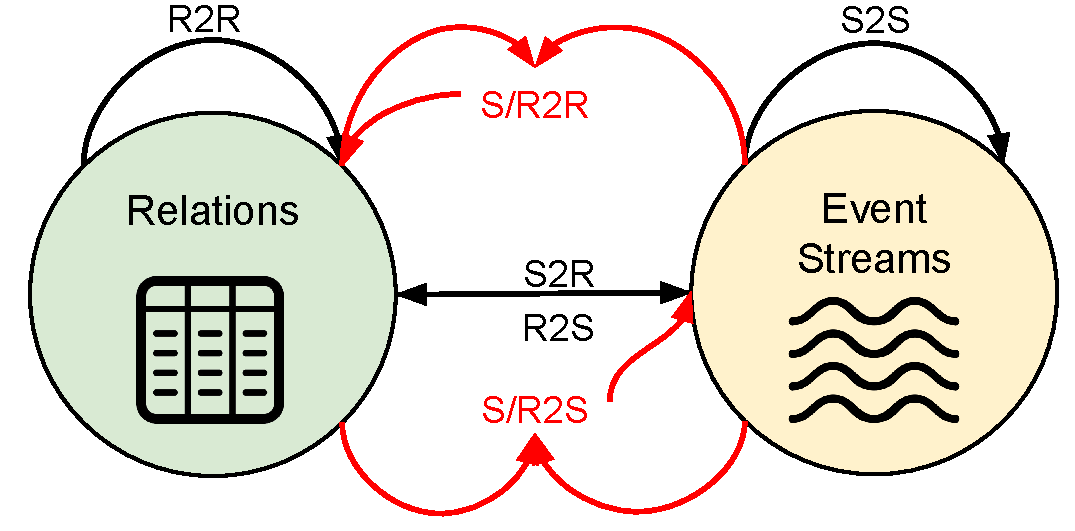
\includegraphics[width=0.55\linewidth]{StreamtoRelation.pdf}
    \caption{The CQL conceptual model: four operator families transform data between streams
    and relations~\cite{DBLP:conf/dbpl/ArasuBW03}.}
    \label{fig:CQL:model}
\end{figure}

Mixed-input families extend this base. A stream element can be enriched against a relation (a stream--relation join), with the result either updating a relation (S/R2R) or emitted onto a stream (S/R2S). Together, the S2R, R2S, S/R2R, and S/R2S families realise the \emph{stream--table duality}~\cite{sax2018streams}: stream elements upsert into an append-only relation, yielding a queryable snapshot of current state at any instant, while that relation, scanned in arrival order, replays the originating stream. This duality is the conceptual core of our approach; Section~\ref{sec:overview} instantiates it for our multi-camera tracking.

Table~\ref{tab:cql:engine:support} summarises stream-management engines and their support for CQL syntax and operator families. We adopt the operator-family taxonomy from our prior
formulation of streams-and-tables for process orchestration~\cite{awad2025best} and re-target
it from process enactment to the perception domain. We select Esper because of: full CQL operator support in an embeddable, single-process JVM runtime, which in the MCOT setting additionally avoids serialising high-dimensional feature tensors across distributed workers (Section~\ref{sec:overview:realisation}). The generated EPL is otherwise portable to other CQL-compliant engines.

\begin{table}[tbh!]
    \centering
    \caption{CQL-compliant engines: operator-family support analysis.}
    \label{tab:cql:engine:support}
    \resizebox{\linewidth}{!}{
    \begin{tabular}{@{}lcccccccc@{}}
        \toprule
        \textbf{Engine} & \textbf{CQL Syntax} & \textbf{S2S} & \textbf{S2R} & \textbf{R2R} & \textbf{R2S} & \textbf{S/R2S} & \textbf{S/R2R} & \textbf{Status} \\
        \midrule
        \multicolumn{9}{c}{\textit{True CQL-compliant engines}} \\
        Stanford STREAM~\cite{DBLP:journals/debu/ArasuBBDIMNSTVW03} & Yes & Yes & Yes & Yes & Yes & Partial & Partial & Discontinued \\
        Esper (EPL) & Yes & Yes & Yes & Yes & Yes & Yes & Yes & Active \\
        Oracle Event Processing~\cite{alves2013getting} & Yes & Yes & Yes & Yes & Yes & Yes & Yes & Active \\
        Apache Flink~\cite{apacheflink} & Yes & Yes & Yes & Yes & Yes & Yes & Yes & Active \\
        Apache Kafka Streams~\cite{DBLP:conf/edbt/JafarpourD19} & No & Yes & Yes & Yes & Yes & Yes & Yes & Active \\
        \midrule
        \multicolumn{9}{c}{\textit{SQL-based streaming (non-CQL compliant)}} \\
        Apache Spark Streaming~\cite{DBLP:conf/sigmod/ArmbrustDTYZX0S18} & No & Yes & Yes & Yes & Yes & Yes & Yes & Active \\
        Apache Samza~\cite{10.14778/3137765.3137770} & No & Yes & Yes & Yes & Yes & Yes & Yes & Active \\
        Apache Storm~\cite{apachestorm} & No & Yes & Yes & Yes & Yes & No & No & Active \\
        \bottomrule
    \end{tabular}
    }
\end{table}





\subsection{Reference Pipeline}
\label{sec:background:baseline}

As a concrete, representative instance of the monolithic architecture above, we take a state-of-the-art batch MCOT pipeline (OSC~\cite{yoshida2024overlap}), developed for
\emph{multi-camera people tracking} (MCPT), the person-specific instantiation of MCOT used throughout the AI City Challenge~\cite{wang2024aicity}; we use MCPT below only when referring to this concrete pipeline and its stages.

The pipeline comprises four stages: per-camera tracklet construction (single-camera tracking), representative feature selection per track, cross-camera re-identification via similarity-based clustering, and a low-confidence detection assignment pass. Our work preserves this functional intent stage-for-stage while re-architecting it as a streams-and-tables operator graph  (Section~\ref{sec:overview}), so that tracklet state and identity mappings are maintained in queryable relational tables rather than buried in pipeline
code.

\section{Related Work}\label{sec:related}

\paragraph{Multi-Camera People Tracking: AI City Challenge Baselines.}
The NVIDIA AI City Challenge~\cite{wang2024aicity} has catalysed the development of high-performing MCPT systems. In the 2024 edition (Track~1), the highest-scoring offline entry by Yoshida et al.~\cite{yoshida2024overlap} (RIIPS/Yachiyo, achieving the highest raw HOTA of 71.94\%) proposed an \emph{offline} framework built on a custom \emph{Overlap Suppression Clustering} (OSC) algorithm. OSC leverages future-frame context to retrospectively resolve overlap anomalies---cases where a single tracklet erroneously contains detections from multiple identities occupying the same frame---using weighted degree centrality for bipartite re-assignment. For cross-camera Re-ID, they categorize detections into three confidence levels (Lv.3/2/1) based on HRNet pose estimation keypoints, select representative images from the highest available level, and cluster them via average-linkage hierarchical clustering on a similarity matrix refined by world-coordinate Euclidean distances. Low-identifiability tracklets are assigned to existing clusters as a final post-processing step. Our system takes this exact pipeline as the functional baseline and re-architects it as a streaming program, achieving 100\% Global ID parity and $<10^{-6}$ MAD in similarity matrices \emph{online}, without requiring offline post-processing.

Among online challenge entrants, Kim et al.~\cite{kim2024cluster} (Nota, 3rd place, with a raw HOTA score of 60.93\%) proposed \emph{Cluster Self-Refinement} (CSR), which periodically executes agglomerative clustering to split tracklets contaminated with mixed-identity features, and merges duplicate global IDs by comparing spatial-visual distances. They further leverage RTMPose for angle-aware ground-plane projection (updating camera-specific interpolation ratios via exponential moving average) and filter occluded bounding boxes via Procrustes shape analysis to ensure diverse, high-quality appearance features in each tracklet. Xie et al.~\cite{xie2024robust} (SJTU-Lenovo, 2nd place in raw HOTA score of 67.22\% but the overall Track~1 winner after the 10\% online tracking bonus) combined geometric consistency constraints with state-aware Re-ID correction to handle camera handoffs. Specker~\cite{specker2024ocmctrack} (OCMCTrack, 4th place, with a raw HOTA score of 60.88\%) introduced a corrective matching cascade consisting of track splitting (to prune false-positive associations based on visual similarity thresholds), position-based hierarchical clustering, adapted projection-line matching (to handle bounding boxes truncated at frame borders), and Re-ID-based rematching for lost tracks. Yang et al.~\cite{yang2024online} (UW-ETRI, 5th place, raw HOTA score of 57.14\%) decoupled spatial association (clustering multi-camera foot-point projections) from temporal tracking (world-coordinate Kalman filtering), but relied heavily on offline post-processing---tracklet splitting via inner cosine feature distance and hierarchical merging---to correct cumulative online errors.

Unlike these approaches, \textbf{STREAMTRACK} does not employ global per-frame bipartite matching cascades or separate offline correction passes. Instead, we express the association logic as continuous SQL/EPL queries over relational state tables (\texttt{GlobalIDTable}, \texttt{CameraTopologyTable}). Identity switches and stale tracks are resolved incrementally via priority-ordered EPL timer queries, and the search space is pruned from global $O(N^2)$ comparisons to $O(N)$ locally via topology-aware stream joins---preserving absolute functional accuracy while delivering a 9.8$\times$ overall speedup over an equivalent JVM batch baseline.

\paragraph{Online vs.\ Offline Tracking and Scalability.}
Multi-camera tracking systems are broadly classified as \emph{offline} (batch) or \emph{online} (incremental). Offline methods~\cite{yoshida2024overlap} leverage global optimization over entire video sequences, exploiting future frames for higher accuracy but at latencies that preclude real-time deployment. Online methods~\cite{kim2024cluster,xie2024robust,specker2024ocmctrack} process observations causally, yet even these ``online'' solutions typically rely on internal batch windows for cross-camera association, accumulating detections over fixed intervals before performing global clustering. Critically, \emph{scalability} in the MCPT literature is almost exclusively treated as a computer-vision concern (handling denser crowds, more detections) rather than a \emph{systems} concern (adding cameras, reconfiguring topology, maintaining state under growth). Our work is orthogonal to these accuracy-centric advances: we take an existing offline pipeline and re-architect it as a streaming program, preserving its functional output while gaining systems-level properties---scalability via topology-aware partitioning ($4.16\times$ latency reduction at 9 cameras, or $4.27\times$ in steady state), inspectability via queryable state tables, and reconfigurability via live topology updates (337\,ms outage, 190\,ms recovery, with zero downtime).

\paragraph{Industrial Video Analytics Frameworks.}
NVIDIA DeepStream~\cite{nvidia2024deepstream} is the dominant industrial SDK for GPU-accelerated video analytics. Built on GStreamer, it provides a modular pipeline of hardware-accelerated plugins for decoding, inference, and single-camera tracking (NvDCF, DeepSORT, IOU). However, its native trackers operate within a single camera stream; cross-camera identity association requires an external microservice layer. NVIDIA Metropolis~\cite{nvidia2025metropolis} addresses this gap with a Kubernetes-based reference architecture that decomposes multi-camera tracking into containerized microservices communicating via message brokers. While Metropolis provides a scalable deployment model, it remains a heavyweight, opaque infrastructure: association logic is embedded in compiled services rather than expressed as declarative queries, intermediate tracking state is not directly queryable for debugging, and reconfiguring the camera network typically requires container re-deployment or manual API calls rather than a single streaming event. In contrast, \textbf{STREAMTRACK} expresses association as parameterized SQL/EPL joins over a relational topology table, enabling zero-downtime reconfiguration, SQL-based state inspection, and a lightweight single-process deployment.

\paragraph{Stream Processing Foundations and CEP Engine Selection.}
Our architectural approach draws from the streams-and-tables duality formalized by Sax et al.~\cite{sax2018streams}. Apache Kafka~\cite{kreps2011kafka} and Apache Flink~\cite{carbone2015flink} provide distributed stateful stream processing with exactly-once guarantees and fault tolerance. While these platforms are well suited for data-parallel workloads, our MCOT setting---where high-dimensional appearance tensors must be shared between tracking operators and relational state---benefits from a single-process, zero-copy approach.

Our implementation uses Esper~\cite{espertech2024}, a mature CEP engine that combines SQL-like continuous queries (EPL) with full relational table semantics in an embeddable, single-process JVM runtime. By running within the application process, Esper enables zero-overhead sharing of appearance feature tensors between tracking operators and state tables, avoiding the cross-process data-movement costs of a distributed design. Esper's API further supports compiling, deploying, and undeploying EPL statements at runtime, which directly enables our reactive topology reconfiguration loop.

The closest prior work applying CEP to video analytics is VidCEP~\cite{yadav2019vidcep}, which introduced a graph-based Video Event Knowledge Graph (VEKG) and a Video Event Query Language (VEQL) for detecting spatiotemporal patterns (e.g., ``Red Car Left of Person'', loitering, traffic flow) in video streams. As analyzed in VidCEP, existing Event Query Languages (such as Snoop~\cite{chakravarthy1994snoop}, SASE~\cite{wu2006sase}, TESLA~\cite{cugola2010tesla}, and Cayuga~\cite{demers2007cayuga}) are designed for temporal sequence matching on alphanumeric event streams and lack the ability to process high-dimensional video streams or reason about spatial relationships. On the other hand, database-oriented video query languages (such as VSQL~\cite{10.1145/951676.951682}, MOQL~\cite{li1997moql}, BilVideo~\cite{donderler2005bilvideo}, SVQL~\cite{lu2015svql}, and CVQL~\cite{le2008query}) support object, attribute, and spatial relationship queries, but are strictly built for batch querying of offline, pre-annotated databases, failing to handle continuous, real-time streaming joins. VidCEP addresses this by extending Esper with external deep learning frameworks to populate a graph-based event model. However, VidCEP targets \emph{post-tracking event and anomaly detection}---recognizing high-level behavior patterns from already-segmented and tracked object trajectories---rather than the structurally distinct problem of \emph{multi-camera identity tracking (MCOT)}. MCOT requires continuously maintaining a mutable table of active identity mappings (\texttt{GlobalIDTable}), resolving coordinate projections, and executing topology-aware joins in real time. We choose Esper because it serves as a high-performance relational coordinator: we do not attempt to represent raw pixels or neural network inference inside the declarative query language itself; rather, we offload vision kernels (Re-ID, projection) to modular operators and use Esper to orchestrate stream windowing, relational state maintenance, and topological gating. To our knowledge, no prior work has applied the streams-and-tables paradigm to the core MCOT pipeline itself.

\paragraph{Summary and Gap.}
The literature reveals a clear gap at the intersection of multi-camera tracking and stream processing systems. CV-oriented works~\cite{yoshida2024overlap,kim2024cluster,xie2024robust,specker2024ocmctrack,yang2024online} focus on improving tracking heuristics but treat the processing architecture as a fixed implementation detail. Industrial frameworks~\cite{nvidia2024deepstream,nvidia2025metropolis} provide scalable deployment but lack declarative association logic, queryable state, and zero-downtime reconfigurability. Stream processing systems~\cite{sax2018streams,carbone2015flink,kreps2011kafka} and video CEP frameworks~\cite{yadav2019vidcep} provide theoretical and practical foundations for continuous data processing but have not been applied to the core MCOT pipeline. \textbf{STREAMTRACK} bridges this gap by formulating multi-camera tracking as a relational streaming program in which identity is a continuously maintained table, association is a parameterized stream join, and the camera topology is a reconfigurable state relation.


\section{Architecture}\label{sec:overview}

\textbf{STREAMTRACK} instantiates the stream--table duality
(Section~\ref{sec:stream:table:duality}) for multi-camera tracking by mapping the three CQL primitives directly onto the tracking problem (Figure~\ref{fig:duality}). \emph{Streams} carry immutable observations, per-camera detections and incremental tracklet updates. \emph{Tables} hold mutable state, the global identity mapping (\texttt{GlobalIDTable}) and the camera-network topology (\texttt{CameraTopologyTable}). \emph{Continuous queries} bridge them, consuming detection streams, reading and updating these tables, and emitting a derived \texttt{GlobalPersonEvent} stream. Casting MCOT in these terms, rather than as a bespoke imperative pipeline, is what makes the system inspectable, reconfigurable, and scalable.

\begin{figure}[tbh!]
\centering
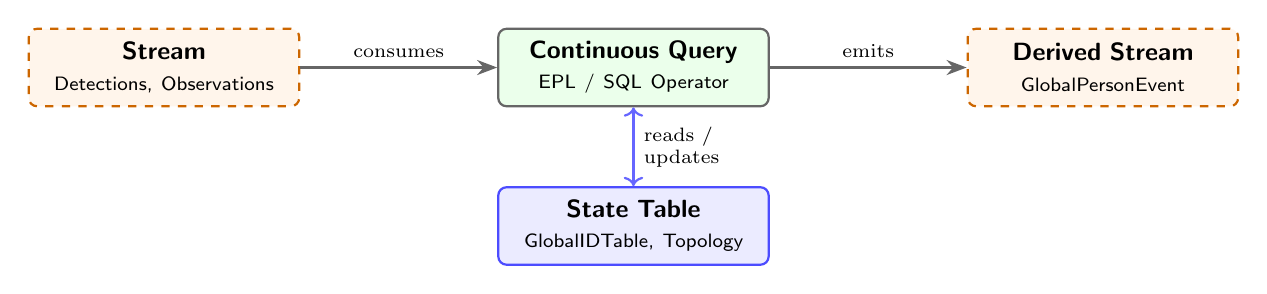
\begin{tikzpicture}[
    node distance=1.8cm and 2.5cm,
    font=\small\sffamily,
    streambox/.style={rectangle, draw=orange!80!black, fill=orange!8, rounded corners=3pt, minimum height=2.8em, text width=3.2cm, align=center, thick, dashed},
    tablebox/.style={rectangle, draw=blue!70, fill=blue!8, rounded corners=3pt, minimum height=2.8em, text width=3.2cm, align=center, thick},
    querybox/.style={rectangle, draw=black!60, fill=green!8, rounded corners=3pt, minimum height=2.8em, text width=3.2cm, align=center, thick},
    arr/.style={-{Stealth[scale=1.1]}, thick, draw=black!60}
]
\node[streambox] (s1) {\textbf{Stream}\\\scriptsize Detections, Observations};
\node[querybox, right=of s1] (q) {\textbf{Continuous Query}\\\scriptsize EPL / SQL Operator};
\node[streambox, right=of q] (s2) {\textbf{Derived Stream}\\\scriptsize GlobalPersonEvent};
\node[tablebox, below=1cm of q] (t) {\textbf{State Table}\\\scriptsize GlobalIDTable, Topology};
\draw[arr] (s1) -- node[above, font=\scriptsize] {consumes} (q);
\draw[arr] (q) -- node[above, font=\scriptsize] {emits} (s2);
\draw[arr, <->, draw=blue!60] (q) -- node[right, font=\scriptsize, align=left] {reads /\\updates} (t);
\end{tikzpicture}
\caption{\textbf{STREAMTRACK}'s streams-and-tables instantiation of MCOT. Detection streams feed continuous EPL/SQL queries that maintain the \texttt{GlobalIDTable} and
\texttt{CameraTopologyTable} as relational state and emit the derived
\texttt{GlobalPersonEvent} stream.}
\label{fig:duality}
\end{figure}

The architecture is organised as a pipeline of continuous operators over detection streams and relational state tables, shown end-to-end in Figure~\ref{fig:architecture}. The same operator graph serves a single camera or an arbitrary camera network: per-camera operators (Section~\ref{sec:single}) produce local tracklet results, and cross-camera operators (Section~\ref{sec:multi}) associate them into global identities. This section specifies~\emph{what} each operator is, its inputs, outputs, processing logic, and CQL operator family, while Sections~\ref{sec:single} and~\ref{sec:multi} detail \emph{how} the single- and multi-camera stages are realised.

% \begin{figure}[tbh!]
% \centering
% \resizebox{\linewidth}{!}{
% \begin{tikzpicture}[
%     node distance=1.2cm and 1.5cm,
%     font=\small\sffamily,
%     block/.style={rectangle, draw=black!70, fill=blue!10, rounded corners=2pt, minimum height=3em, text width=2.6cm, align=center, thick},
%     table/.style={cylinder, shape border rotate=90, aspect=0.25, draw=black!70, fill=gray!15, text width=2.4cm, align=center, minimum height=3.5em, thick},
%     arrow/.style={-{Stealth[scale=1.2]}, thick, draw=black!70},
%     stream/.style={-{Stealth[scale=1.2]}, thick, draw=orange!80!black, dashed},
%     group_box/.style={rectangle, draw=black!50, rounded corners=4pt, inner sep=10pt, dashed}
% ]

% % Nodes
% \node[block] (ingest) {Ingestion \& \\ Feat. Enrich};
% \node[block, right=of ingest] (scpt) {Windowed Single \\ Camera Tracking};
% \node[block, right=of scpt] (join) {Topology-Aware \\ Stream Join};
% \node[block, right=of join] (mcpt) {Rep. Selection \\ \& HAC Cluster};
% \node[block, right=of mcpt] (global) {Global Identity \\ Maintenance};

% \node[table, above=0.8cm of join] (topology) {CameraTopology\\Table};
% \node[table, above=0.8cm of mcpt] (calibration) {Calibration\\Table};
% \node[table, above=0.8cm of global] (globaltable) {GlobalIDTable};

% % Arrows
% \draw[stream] ($ (ingest.west) - (1cm,0) $) -- node[above] {\scriptsize Detections} (ingest.west);
% \draw[arrow] (ingest) -- node[above] {\scriptsize stream} (scpt);
% \draw[arrow] (scpt) -- node[above, align=center] {\scriptsize SingleCam\\ \scriptsize Result} (join);
% \draw[arrow] (join) -- node[above, align=center] {\scriptsize Synced\\ \scriptsize Group} (mcpt);
% \draw[arrow] (mcpt) -- node[above] {\scriptsize Updates} (global);

% % State connections
% \draw[arrow, dashed, draw=blue!60] (topology) -- node[right] {\scriptsize reads} (join);
% \draw[arrow, dashed, draw=blue!60] (calibration) -- node[right] {\scriptsize reads} (mcpt);
% \draw[arrow, dashed, draw=blue!60, <->] (globaltable) -- node[right, align=left] {\scriptsize merge/delete\\ \scriptsize (TrackExpired)} (global);

% % Group background
% \begin{scope}[on background layer]
%     \node[group_box, fit=(join) (mcpt), fill=green!5, label={[anchor=base, inner sep=0pt, font=\scriptsize\bfseries\sffamily]above:Cross-Camera Association}] {};
% \end{scope}

% \end{tikzpicture}
% }
% \caption{STREAMTRACK Operator Graph. Detections arrive as streams from individual cameras. Single-camera tracking is a stateful stream operator. Cross-camera association uses a topology-aware stream join, parametrised by the \texttt{CameraTopologyTable}, before performing global appearance clustering. State tables enable memory-safe, time-bounded identity maintenance.}
% \label{fig:architecture}
% \end{figure}

\begin{figure*}[tbh!]
\centering
\resizebox{\textwidth}{!}{
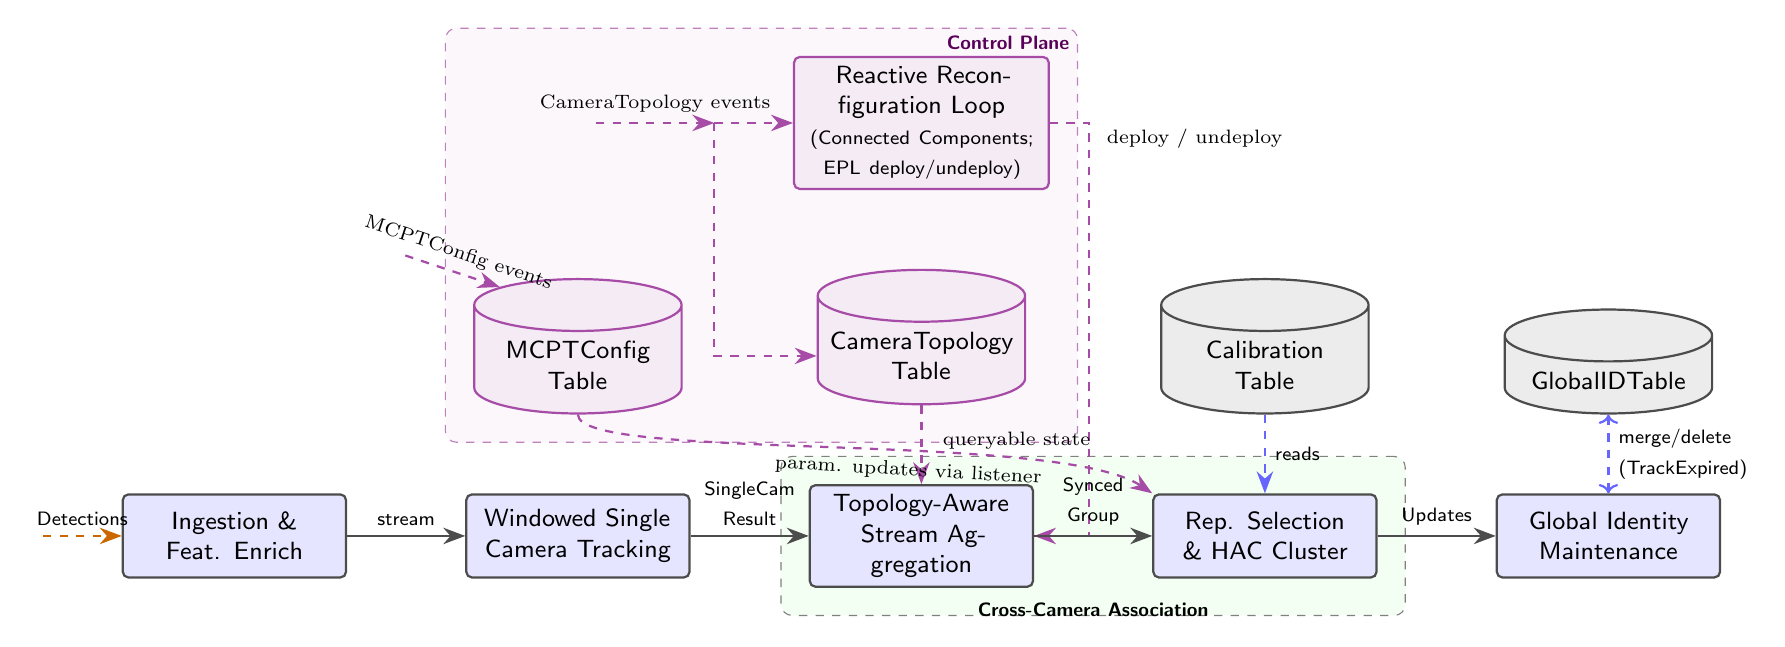
\begin{tikzpicture}[
    node distance=1.2cm and 1.5cm,
    font=\small\sffamily,
    block/.style={rectangle, draw=black!70, fill=blue!10, rounded corners=2pt, minimum height=3em, text width=2.6cm, align=center, thick},
    ctrlblock/.style={rectangle, draw=violet!70, fill=violet!8, rounded corners=2pt, minimum height=3em, text width=3.0cm, align=center, thick},
    table/.style={cylinder, shape border rotate=90, aspect=0.25, draw=black!70, fill=gray!15, text width=2.4cm, align=center, minimum height=3.5em, thick},
    ctrltable/.style={cylinder, shape border rotate=90, aspect=0.25, draw=violet!70, fill=violet!8, text width=2.4cm, align=center, minimum height=3.5em, thick},
    arrow/.style={-{Stealth[scale=1.2]}, thick, draw=black!70},
    stream/.style={-{Stealth[scale=1.2]}, thick, draw=orange!80!black, dashed},
    staterw/.style={-{Stealth[scale=1.2]}, thick, draw=blue!60, dashed},
    ctrl/.style={-{Stealth[scale=1.2]}, thick, draw=violet!70, dashed},
    group_box/.style={rectangle, draw=black!50, rounded corners=4pt, inner sep=10pt, dashed}
]
% ---------------- DATA PLANE ----------------
\node[block] (ingest) {Ingestion \& \\ Feat. Enrich};
\node[block, right=of ingest] (scpt) {Windowed Single \\ Camera Tracking};
\node[block, right=of scpt] (join) {Topology-Aware \\ Stream Aggregation};
\node[block, right=of join] (mcpt) {Rep. Selection \\ \& HAC Cluster};
\node[block, right=of mcpt] (global) {Global Identity \\ Maintenance};
\node[table, above=1.0cm of mcpt] (calibration) {Calibration\\Table};
\node[table, above=1.0cm of global] (globaltable) {GlobalIDTable};
% ---------------- CONTROL PLANE ----------------
\node[ctrltable, above=1.0cm of join] (topology) {CameraTopology\\Table};
\node[ctrltable, above=1.0cm of scpt] (configtable) {MCPTConfig\\Table};
\node[ctrlblock, above=1.0cm of topology] (reconfig) {Reactive Reconfiguration Loop\\ \scriptsize (Connected Components; EPL deploy/undeploy)};
% control event streams entering from the left
\draw[ctrl] ($ (configtable.north west) + (-1.2,0.4) $) -- node[above, font=\scriptsize, sloped] {MCPTConfig events} (configtable.north west);
% CameraTopology events: split to two parallel targets
\draw[ctrl] ($ (reconfig.west) + (-2.5,0) $) -- node[above, font=\scriptsize] {CameraTopology events} ($ (reconfig.west) + (-1.0,0) $);
\draw[ctrl] ($ (reconfig.west) + (-1.0,0) $) -- (reconfig.west);
\draw[ctrl] ($ (reconfig.west) + (-1.0,0) $) |- (topology.west);
% control wiring
\path (reconfig.east) ++(0.5,0) coordinate (rjoin);
\draw[ctrl] (reconfig.east) -- (rjoin) |- (join.east);
\path (rjoin) ++(0.1,-0.2) node[right, font=\scriptsize] {deploy / undeploy};
% table read by aggregation queries
\path (topology.south) ++(0,-0.45) coordinate (tjoin);
\draw[ctrl] (topology.south) -- (tjoin) -| (join.north);
\path (tjoin) ++(0.15,0) node[right, font=\scriptsize] {queryable state};
\draw[ctrl] (configtable.south) .. controls +(0,-0.6) and +(-1.2,0.8) .. node[below, font=\scriptsize, sloped, pos=0.6] {param. updates via listener} (mcpt.north west);
% ---------------- Data-plane arrows ----------------
\draw[stream] ($ (ingest.west) - (1cm,0) $) -- node[above] {\scriptsize Detections} (ingest.west);
\draw[arrow] (ingest) -- node[above] {\scriptsize stream} (scpt);
\draw[arrow] (scpt) -- node[above, align=center] {\scriptsize SingleCam\\ \scriptsize Result} (join);
\draw[arrow] (join) -- node[above, align=center] {\scriptsize Synced\\ \scriptsize Group} (mcpt);
\draw[arrow] (mcpt) -- node[above] {\scriptsize Updates} (global);
\draw[staterw] (calibration) -- node[right] {\scriptsize reads} (mcpt);
\draw[staterw, <->] (globaltable) -- node[right, align=left] {\scriptsize merge/delete\\ \scriptsize (TrackExpired)} (global);
% ---------------- Group backgrounds ----------------
\begin{scope}[on background layer]
    \node[group_box, fit=(join) (mcpt), fill=green!5,
      label={[anchor=base, inner sep=1pt, font=\scriptsize\bfseries\sffamily]below:Cross-Camera Association}] {};
    \node[group_box, draw=violet!50, fit=(reconfig) (configtable) (topology), fill=violet!3,
      label={[anchor=north east, inner sep=3pt, font=\scriptsize\bfseries\sffamily, text=violet!70!black]north east:Control Plane}] {};
\end{scope}
\end{tikzpicture}
}
\caption{\textbf{STREAMTRACK} operator graph with its two planes. The \emph{data plane}
(bottom) preserves the functional structure of the reference pipeline: detections arrive as
per-camera streams, single-camera tracking is a stateful windowed operator, and cross-camera
association aggregates results before global appearance clustering, with the
\texttt{CalibrationTable} and \texttt{GlobalIDTable} as relational state. The \emph{control
plane} (top, violet) carries the operational contribution: \texttt{CameraTopology} and
\texttt{MCPTConfig} events upsert into control tables (which serve as queryable state for the
operators below), and a reactive reconfiguration loop watches the \texttt{CameraTopology}
event stream, recomputes connected components, and deploys or undeploys association queries
at runtime---so both the network topology and the algorithmic parameters are reconfigurable as
data, with zero downtime.}
\label{fig:architecture}
\end{figure*}
 
% ============================================================
% Accompanying prose: INSERT immediately after the paragraph in
% Section 3 that introduces fig:architecture ("The architecture is
% organised as a pipeline of continuous operators ... realised.").
% ============================================================
 
The operator graph separates two concerns. The \emph{data plane}---ingestion, single-camera
tracking, cross-camera association, clustering, and identity maintenance---mirrors the
reference pipeline (Section~\ref{sec:background:baseline}) stage for stage; this is what makes
functional parity with the state-of-the-art baseline achievable by construction
(Section~\ref{sec:eval:parity}). The \emph{control plane} is where the architectural gains
live: \texttt{CameraTopology} and \texttt{MCPTConfig} events are themselves streams that
upsert into control tables, and a reactive reconfiguration loop watches the
\texttt{CameraTopology} event stream directly, recomputes the connected components of the
neighbourhood graph, and redeploys the affected association queries at runtime. Operational
concerns---which cameras are grouped, which thresholds apply, when queries are rebuilt---are
thus expressed in the same streams-and-tables vocabulary as the tracking itself, rather than
in configuration files or code. The data plane
answers \emph{what the baseline computes}; the control plane answers \emph{how the deployment
adapts}, and it is the latter that delivers the scalability, inspectability, and
reconfigurability properties claimed in Section~\ref{sec:background:mcot}.
% TODO[Student[done]]: verify the control-plane wiring against the implementation:
% (1) Do CameraTopology events flow through the reconfiguration loop into the table (as drawn),
%     or directly into the table with the loop as a listener? Adjust the arrow direction if needed.
% (2) Confirm MCPTConfig updates are applied via a listener on MCPTConfigTable and read by the
%     MCPT kernel per invocation, as stated in the runtime-parameter paragraph of the evaluation.
% (3) Provide the actual EPL for the MCPTConfigTable upsert (mirroring the CameraTopologyTable
%     on-merge statement) for Section 5 or an appendix.
% (1) CameraTopology events flow in PARALLEL: the on-merge upsert goes directly into
%     CameraTopologyTable (IotMain.prepareTopologyQueries), while a separate `select * from
%     CameraTopology` listener (IotMain.multiCameraAggregationQueries) triggers the reactive
%     reconfiguration loop (topologyGraph update -> computeClusters -> deploy/undeploy
%     aggregation EPL). The loop does NOT interact with CameraTopologyTable; the figure now
%     reflects this with a split entry path.
% (2) MCPTConfig updates are applied via a `select * from MCPTConfig` listener that calls
%     applyRuntimeParameter(), which reflectively updates TrackingParameters statics. The MCPT
%     kernel reads these statics per invocation (passed as method args from
%     processAggregatedResults). There is no listener on MCPTConfigTable itself; the table
%     serves as a queryable side-effect of the on-merge upsert.
% (3) The MCPTConfigTable upsert EPL mirrors the CameraTopologyTable pattern:
%       on MCPTConfig as cfg
%       merge into MCPTConfigTable as target
%       where target.paramName = cfg.paramName
%       when matched then
%         update set target.paramValue = cfg.paramValue, target.paramType = cfg.paramType
%       when not matched then
%         insert select cfg.paramName as paramName, cfg.paramValue as paramValue, cfg.paramType as paramType;
%     See IotMain.prepareConfigQueries().

\subsection{Operator Model}
\label{sec:overview:operatormodel}
Every operator in \textbf{STREAMTRACK} is specified uniformly by the streams and tables it consumes, the stream or table it produces, its processing logic, and the CQL operator
family it belongs to. Table~\ref{tab:operatormodel} gives this specification for the full pipeline; the streams and state tables it references are defined below.%\todo{student[Done]: Review the streams in/out in Table~\ref{tab:operatormodel} correct if necessary}

\begin{table*}[tbh!]
    \centering
    \caption{The \textbf{STREAMTRACK} operator model. Each operator is specified by the streams and tables it consumes, what it produces, its processing logic, and the CQL operator family it realises. Vision kernels (Re-ID embedding, homography projection, HAC) are treated as black-box UDFs invoked by the operators; the streams-and-tables layer performs the relational
    coordination.}
    \label{tab:operatormodel}
    \small
    \setlength{\tabcolsep}{4pt}
    \renewcommand{\arraystretch}{1.25}
    \begin{tabularx}{\textwidth}{@{} l X X X c @{}}
        \toprule
        \textbf{Operator} & \textbf{Input (stream / table)} & \textbf{Output} & \textbf{Processing logic} & \textbf{CQL} \\
        \midrule
        Ingestion \& Feature Enrichment
            & raw detections
            & \texttt{embeddingFeature} (stream)
            & Project and attach Re-ID embedding
            & S2S \\
        \addlinespace
        Single-Camera Tracking
            & \texttt{embeddingFeature} (stream)
            & \texttt{SingleCameraResult} (stream)
            & Windowed frame-to-frame association and post-processing (sNMS, warp, short-track exclusion)
            & S2R\,$\to$\,R2S \\
        \addlinespace
        Topology-Aware Association
            & \texttt{SingleCameraResult} (stream)
            & synced cross-camera group (stream)
            & Windowed stream aggregation parameterised by topology
            & S2R\,$\to$\,R2S \\
        \addlinespace
        Representative Selection
            & synced group (stream); \texttt{CalibrationTable}
            & \texttt{GlobalPersonEvent} (stream)
            & Keypoint/centrality selection; homography enrichment and clustering (MCPT)
            & S/R2S \\
        \addlinespace
        Global Identity Maintenance
            & \texttt{GlobalPersonEvent} (stream); \texttt{GlobalIDTable}
            & updated \texttt{GlobalIDTable}
            & Upsert (\texttt{MERGE}); materialise identity view
            & S/R2R \\
        \addlinespace
        Track Expiry \& Eviction
            & \texttt{GlobalIDTable} (timer)
            & \texttt{TrackExpiredEvent} (stream)
            & Staleness scan; emit and delete stale rows
            & R2S\,/\,R2R \\
        \bottomrule
    \end{tabularx}
\end{table*}

% TODO(confirm)[Done]: consolidated Operator Model table replacing tab:dag + reflection prose.

\paragraph{Streams}
\begin{itemize}[leftmargin=*]
    \item $\texttt{embeddingFeature}(\textit{cameraId}, \textit{curFrame}, \textit{timestamp}, \textit{detectedUsers}[])$
    \item $\texttt{SingleCameraResult}(\textit{cameraId}, \textit{windowIndex}, \textit{clusterLabels}[], \textit{featureList}[], \textit{frameNumbers}[], \textit{timestamps}[], \dots)$
    \item $\texttt{GlobalPersonEvent}(\textit{globalId}, \textit{cameraId}, \textit{serial}, \textit{localId}, \textit{x}, \textit{y}, \textit{timestamp}, \textit{attributes}\{\})$
    \item $\texttt{TrackExpiredEvent}(\textit{globalId})$
\end{itemize}

\paragraph{State Tables%\todo{student[Done]: align the stream names and table names with what in Table~\ref{tab:operatormodel}}
}
\begin{itemize}[leftmargin=*]
    \item $\texttt{GlobalIDTable}(\textit{globalId}, \textit{lastSeen}, \textit{attributes}\{\textit{Cameras}[], \textit{Timestamp}, \textit{Coordinate}\})$
    \item $\texttt{CalibrationTable}(\textit{cameraId}, \textit{homographyMatrix})$
    \item $\texttt{CameraTopologyTable}(\textit{cameraId}, \textit{neighborId}, \textit{enabled}, \textit{overlapping})$
\end{itemize}

Mapping%\todo{student[Done]: review the following part. For example, I am not sure if cross-camera association is stream-to-stream or stream-to-relation join. Read carefully and correct based on what you have done} 
~these operators onto the CQL families makes the duality concrete and shows that each MCOT challenge from Section~\ref{sec:background:mcot} is addressed by a specific operator class. Ingestion and feature enrichment are stateless stream-to-stream (S2S) mappings. Single-camera tracking pairs a stream-to-relation (S2R) window operator with a relation-to-stream (R2S) emission of \texttt{SingleCameraResult}. Cross-camera association is realised as a topology-parametrised stream aggregation (S2R\,$\to$\,R2S): the \texttt{SingleCameraResult} stream is grouped and synchronised across cameras using a windowed time-batch and a dynamic \texttt{IN(\dots)} camera-group filter, with the active query graph automatically redeployed by a reactive topology manager whenever the network topology changes. This directly addresses the \emph{scalable-association} and \emph{reconfiguration} challenges. Global identity maintenance writes each \texttt{GlobalPersonEvent} into the \texttt{GlobalIDTable} via a stream--relation merge
(S/R2R), continuously materialising the identity view, the \emph{inspectable-state} challenge, while a priority-ordered timer query emits \texttt{TrackExpiredEvent} (R2S) and evicts stale rows (R2R). The \texttt{GlobalIDTable} is thus both a queryable snapshot of identity and a replayable event
source: the stream--table duality in operation.

\subsection{Execution Semantics}
\label{sec:overview:execution}

Operators are evaluated continuously as new tuples arrive, i.e., new camera frames. Windows and joins use ingestion timestamps $\textit{ts\_ingest}$. State tables maintain current hypotheses, i.e., the assigned object ID, and apply eviction rules based on ingestion-time staleness (e.g., tracklet inactivity).

% Append this as the CLOSING subsection of Section 3 (Architecture),
% AFTER \subsection{Execution Semantics}. It absorbs the cross-cutting,
% engine-level parts of the old Implementation section.

\subsection{Realisation on Esper}
\label{sec:overview:realisation}
The operator model above is engine-agnostic: any CQL-compliant engine (Section~\ref{sec:stream:table:duality}) could host it. We realise it on Esper, whose EPL language provides every operator family together with first-class relational tables, and whose embeddable single-process runtime suits the tensor-heavy MCOT setting. Sections~\ref{sec:single} and~\ref{sec:multi} give the per-operator EPL; here we state the engine-level rationale and the conventions shared across all operators.


\paragraph{Why SQL-first on a CEP engine}
Implementing MCOT via SQL/EPL on an embeddable complex-event-processing engine such as Esper~\cite{espertech2024} offers four systems-level advantages that are particularly relevant in the tensor-heavy MCOT setting:
\begin{itemize}[leftmargin=*]
    \item \textbf{Embeddable JVM-local runtime.} Esper is a lightweight library running inside the application process, enabling zero-copy sharing of appearance tensors between tracking operators and relational state in memory, without any inter-process serialisation overhead.
    \item \textbf{Relational state-table semantics.} Esper provides first-class relational tables with primary keys, indexes, and continuous transactional merges (EPL \texttt{MERGE}). This lets us model the active camera neighbourhood and global identity mappings as queryable relations that can be inspected at runtime.
    \item \textbf{Deterministic memory and tensor management.} Esper allows priority-annotated temporal queries (e.g., \texttt{TrackExpiredEvent}) that evict stale \texttt{GlobalIDTable} rows and trigger immediate JVM garbage collection of heavy vision tensors after a configurable inactivity window.
    \item \textbf{Zero-downtime topology reconfiguration.} Esper compiles, deploys, and undeploys EPL statements at runtime, so our reactive loop installs updated topological joins on-the-fly when \texttt{CameraTopology} events arrive, without interrupting tracking.
\end{itemize}
Unlike database-oriented video query systems (e.g., MOQL~\cite{li1997moql}, BilVideo~\cite{donderler2005bilvideo}, SVQL~\cite{lu2015svql}), built for static repositories, and pure pattern-matching CEP systems (e.g., Snoop~\cite{chakravarthy1994snoop}, SASE~\cite{wu2006sase}, TESLA~\cite{cugola2010tesla}), which lack mutable indexed state, Esper uniquely unites stream windowing/joins with queryable relational tables in one engine.

\paragraph{Modular operator design}
The architecture is functionally modular, akin to interchangeable ``Lego-like'' blocks. By decoupling the temporal stream-routing logic (EPL) from the heavy tracking kernels, the system permits seamless algorithm substitution. Esper handles stream synchronisation, windowing, and topological joining; when a window fills, it triggers a listener that dispatches the collected data to a native tracking operator (Figure~\ref{fig:architecture}). A developer can swap the clustering kernel (e.g., replace the default agglomerative clusterer with a density-based or deep classifier) by updating the listener registration at the engine--kernel boundary, evolving the vision logic without redesigning ingestion or synchronisation.

\paragraph{Ordering and jitter under ingestion time}
Ingestion-time semantics avoid the complexity of event-time watermarking. To absorb out-of-order delivery and jitter, the system uses a timeout-bounded aggregation window (e.g., \texttt{win:time(...) group by windowIndex having count(*) = numCameras}): the aggregation advances either when all participating cameras have reported for a \texttt{windowIndex}, or when the maximum latency expires, guaranteeing a predictable progress rate even if a camera fails to report.
% TODO(consistency)[Done]: the synchronisation window literal here must match the per-operator EPL
% (currently win:time(2 min)) and the "3-second" figure in the evaluation. Reconcile all three.
% Note: the system uses two distinct temporal parameters:
% (1) The single-camera tracking window is 3 seconds (90 frames at 30 fps, win:length_batch(90)),
%     which determines the duration of video processed per SCPT cycle.
% (2) The cross-camera aggregation timeout is win:time(2 min), which is the maximum wait for
%     all cameras in a topology group to report before the synchronised window advances.

\paragraph{Configuration parameters.}
Runtime-tunable parameters are exposed via a \texttt{ConfigurationTable}: (i) synchronisation window size (frames), (ii) clustering similarity thresholds, (iii) neighbourhood links in the topology, and (iv) state-eviction TTLs---allowing administrators to tune the accuracy--latency trade-off dynamically.

%====================================================================
% SECTION 4: SINGLE-CAMERA OPERATORS  (Section 6 EPL absorbed per-operator)
%====================================================================
\section{Single-Camera Operators}
\label{sec:single}

These operators run independently per camera. They read only per-camera streams, touch none of the cross-camera state tables, and produce the clean \texttt{SingleCameraResult} stream that the cross-camera layer (Section~\ref{sec:multi}) consumes. This is the \emph{local} half of the two-problem decomposition introduced in Section~\ref{sec:background:mcot}. Each operator below is realised as one or more EPL statements on Esper (Section~\ref{sec:overview:realisation}).

\subsection{Ingestion and Feature Enrichment}
\label{sec:single:ingestion}

This stage ingests per-camera detections and attaches appearance-embedding vectors extracted by a pre-trained Re-ID model, emitting the \texttt{embeddingFeature} stream (a stateless S2S map). For cameras that require world locations, a continuous listener populates the \texttt{CalibrationTable} with per-camera homography matrices at ingestion time. The table is subsequently \emph{read} by the native MCPT clustering kernel (Section~\ref{sec:multi:repselect}), which projects bounding-box foot-points from the 2D image plane to a unified ground-plane coordinate system, enabling spatial gating and distance-based heuristics during cross-camera association. Thus, the \texttt{CalibrationTable} is \emph{maintained} at ingestion but \emph{consumed} downstream, consistent with its attribution to the Representative Selection row in Table~\ref{tab:operatormodel}.


Feature extraction happens at the ingestion boundary, before events enter Esper; each enriched detection is then streamed in under a per-camera event type. The per-camera event types are declared as EPL schemas once at startup:
%TODO[Student[done]]: Put proper EPL staements here.
\begin{verbatim}
-- Per-camera event schema (one per camera, derived from the Java bean)
create schema embeddingFeature_camera_0001 as
    (timestamp long, curFrame int, detectedUsers java.util.List);
\end{verbatim}
Each camera gets its own event type name (\texttt{embeddingFeature\_camera\_0001}, \texttt{...0002}, etc.), which lets the downstream tracking EPL filter by stream name without adding a \texttt{cameraId} predicate to every query.

A continuous listener populates the \texttt{CalibrationTable} at ingestion time so that homography matrices are available to the downstream MCPT kernel:
\begin{verbatim}
-- Define calibration state table
create table CalibrationTable (
    cameraId int primary key,
    homographyMatrix Object
);

-- Populate from incoming CameraCalibration events
insert into CalibrationTable
select cameraId, homographyMatrix from CameraCalibration;
\end{verbatim}
Once per frame, the enriched detections (Re-ID embeddings attached) are streamed into the engine under their camera-specific event type. This is the sole Java-side boundary call (events originate from the file reader, not from another EPL stream):
\begin{verbatim}
// Ingestion boundary: extract features, then send to Esper
EventEPLUtil.streamEvent(
    new EmbeddingFeature(timestamp, frameNumber, detectedUsers),
    "embeddingFeature_camera_0001");
\end{verbatim}

\subsection{Single-Camera Tracking as Stateful Stream Processing}
\label{sec:single:sct}
Single-camera tracking is a stateful windowed operator (S2R\,$\rightarrow$\,R2S). It maintains detection history within a sliding window (e.g., 90--120 frames) to perform frame-to-frame association, aggregating appearance features and keypoint-stability metrics per tracklet, and emits one \texttt{SingleCameraResult} event once the tracklet's window is processed. The window operator is expressed directly in EPL with a length-batch window:
\begin{verbatim}
-- Stateful windowed single-camera tracking
select detectedUsers, curFrame, timestamp
from embeddingFeature_camera_0001.win:length_batch(90)
\end{verbatim}

\subsection{Overlap Suppression}
\label{sec:single:overlap}

Each camera's detection stream is cleaned by an overlap-suppression step that removes redundant, overlapping bounding boxes so that each physical object yields a single best detection rather than several near-duplicate boxes. This is a standard non-maximum suppression (NMS) operation~\cite{neubeck2006efficient} %\todo{student[Done]: cite NMS / the detector's box-suppression method}
applied \emph{independently within a single camera}. In our implementation, a sequential NMS variant suppresses temporally and spatially overlapping detections at the ingestion boundary before events enter the tracking window. As a stateless S2S transformation that consumes detections and emits deduplicated ones, it precedes tracking and improves the quality of the tracklets formed downstream. By removing spurious within-camera duplicates, it also indirectly reduces false candidates entering the cross-camera join. As a detector-side post-processing step, it is applied at the ingestion boundary and has no EPL counterpart. No separate cross-camera duplicate-merge step exists; cross-camera identity resolution is handled entirely by the topology-aware association operators in Section~\ref{sec:multi}.

\paragraph{Disambiguation: overlap suppression vs.\ field-of-view overlap}

Overlap suppression must not be confused with \emph{field-of-view (FoV) overlap}, despite the shared term. Overlap suppression operates on \emph{bounding boxes within a single camera}: it is a detection-level deduplication step. FoV overlap is a \emph{multi-camera deployment property} in which two or more cameras observe the same physical region, possibly from different viewpoints. FoV overlap is a relation \emph{between} cameras, represented explicitly by the \texttt{overlapping} attribute of the \texttt{CameraTopologyTable} (Section~\ref{sec:multi:topology}), where it determines which cameras are grouped into synchronisation joins. The two concepts operate at different levels, pixels within a camera versus visibility across cameras, and are never combined in a single operator.

% TODO(student confirm)[Done]: original text placed suppression "within the core clustering module"
% and mentioned "different cameras". Per the NMS definition this is detection-level and
% single-camera. Confirm exactly where it executes (detector output vs. a separate operator),
% and confirm there is no SEPARATE cross-camera duplicate-merge step. If such a cross-camera
% step exists, it is distinct from NMS and belongs in Section~\ref{sec:multi} under FoV-overlap
% grouping, not here.

%====================================================================
% SECTION 5: CROSS-CAMERA OPERATORS  (Section 6 EPL absorbed per-operator)
%====================================================================
\section{Cross-Camera Operators}
\label{sec:multi}

These operators reason over two or more cameras. They consume the \texttt{SingleCameraResult} stream and read or update the cross-camera relations, \texttt{CameraTopologyTable}, \texttt{CalibrationTable}, and \texttt{GlobalIDTable}, to assign consistent global identities. This is the \emph{global} half of the decomposition, and where the systems-level challenges of Section~\ref{sec:background:mcot} (scalable association, inspectable state, runtime reconfiguration) are answered. As in Section~\ref{sec:single}, each operator is realised as EPL on Esper (Section~\ref{sec:overview:realisation}).

\subsection{Naive Cross-Camera Matching Cost}
\label{sec:multi:naive}
Naive cross-camera association compares tracklets across all camera pairs. For $m$ cameras, each with multiple tracklets, exhaustive matching produces a combinatorial explosion of candidate comparisons, which becomes the primary scalability bottleneck as the network grows, the \emph{scalable-association} challenge in concrete form.

\subsection{Topology-Aware Candidate Generation}
\label{sec:multi:assoc}

We formulate cross-camera association as a topology-parameterised stream-aggregation query synchronised by a \texttt{windowIndex} (an S2R\,$\to$\,R2S operator). By restricting comparisons and aggregations to localised camera groups, the candidate count drops sharply, confirmed by our 9-camera benchmark, where topology-aware partitioning yields a \textbf{4.16$\times$} reduction in per-call latency (up to \textbf{4.27$\times$} in steady state excluding JVM warm-up) relative to global matching (Section~\ref{sec:evaluation}).
%TODO[Student[done]]: This query below shows no joins at all. Is it really used for global ID tracking? Or, are there other statements? Also, where does the knowledge of the cameras 001 and 002, for example, come from? Do they come from the topology table?
Note that the query below contains \emph{no explicit join keyword}---it uses a filter predicate (\texttt{cameraId in (\dots)}) rather than a stream--table join against \texttt{CameraTopologyTable}. This is deliberate. In CQL terms the operator \emph{is} a join: it associates the detection stream with the topology relation to group cameras into synchronised clusters. The physical execution strategy, however, evaluates this join at \emph{plan time} rather than per tuple. The neighbour set is resolved once from the topology table, compiled directly into an \texttt{IN(\dots)} predicate, and baked into the deployed EPL. This is the streaming analogue of partition pruning and constant-expression folding in relational optimisers: because topology changes orders of magnitude less frequently than detections arrive, materialising the join result into the query plan eliminates a per-tuple table probe on the hot path while preserving the relational semantics. The topology relation remains the single source of truth (every deployed predicate is derivable from it), and a topology update becomes a plan change rather than a code change.
\begin{verbatim}
-- Deployed synchronised cross-camera aggregation
-- (one such query per connected component of the topology graph;
--  the IN(...) list is compiled from CameraTopologyTable at plan time)
select window( * ) as results
from SingleCameraResult(cameraId in
    ('camera_0001', 'camera_0002')).win:time(2 min)
group by windowIndex
having count(*) = 2;
\end{verbatim}
The aggregation query is the first half of the identity-tracking path. Once its listener dispatches grouped tracklets to the MCPT kernel, the resulting \texttt{GlobalPersonEvent}s are written into the \texttt{GlobalIDTable} via a separate on-merge statement (Section~\ref{sec:multi:globalid}), and stale entries are evicted by a priority-ordered timer query---these are the actual identity-maintenance statements.

The mechanism that populates the \texttt{IN(\dots)} at plan time is itself expressed in EPL. The topology is stored as a relational table and updated atomically as \texttt{CameraTopology} events arrive:
\begin{verbatim}
-- Define topology state table (composite primary key for adjacency)
create table CameraTopologyTable (
    cameraId string, neighborId string, enabled boolean, overlapping boolean,
    primary key(cameraId, neighborId)
);

-- Atomic upsert from incoming CameraTopology events
on CameraTopology as ct
merge into CameraTopologyTable as target
where target.cameraId = ct.cameraId and target.neighborId = ct.neighborId
when matched then
  update set target.enabled = ct.enabled, target.overlapping = ct.overlapping
when not matched then
  insert select ct.cameraId, ct.neighborId, ct.enabled, ct.overlapping;
\end{verbatim}
A second parallel listener subscribes to the same event stream to detect changes and trigger redeployment---the control-plane half that converts a topology change into a plan change:
\begin{verbatim}
-- Reactive trigger: any CameraTopology event recompiles
-- the affected aggregation queries with updated IN(...) lists.
select * from CameraTopology;
\end{verbatim}
Both statements consume every \texttt{CameraTopology} event in parallel: the on-merge persists the state into the table, while the listener fires \texttt{reconcileDeployments()}, which recomputes the connected components of the graph, diffs them against the currently active deployment set, and for each new or changed component calls \texttt{deployAggregationQuery()}---the method that iterates the camera set, builds the \texttt{IN(\dots)} string, and compiles a fresh EPL statement at runtime. This is the split-entry design visible in Figure~\ref{fig:architecture} (the violet control plane): one event stream, two parallel EPL consumers---one for state, one for reaction.

Because the join result is materialised into the query plan once per topology change rather than re-evaluated for every arriving \texttt{SingleCameraResult} event, a topology update is a plan change, not a code change---the essence of zero-downtime reconfiguration (Section~\ref{sec:multi:topology}).

% TODO(consistency)[Done]: the win:time(2 min) here is the synchronisation window; reconcile with the
% "3-second synchronization window" referenced near the reconfiguration result in the evaluation.
% Note: win:time(2 min) is the cross-camera aggregation timeout (maximum latency for all cameras
% in the group to report). The "3-second" figure in the evaluation refers to the single-camera
% tracking window (90 frames at 30 fps), which is a distinct parameter.

\subsection{Camera Topology as a Reconfigurable State Table}
\label{sec:multi:topology}
A key feature is treating camera neighbourhoods as a relational configuration rather than hardcoded logic. The \texttt{CameraTopologyTable} stores the active neighbour graph, where the \texttt{overlapping} flag marks pairs of cameras with \emph{shared fields of view} (Section~\ref{sec:single:overlap} contrasts this with within-camera overlap suppression). Administrators update the table at runtime by streaming \texttt{CameraTopology} events, and changes take effect for the next window of tracklets. This tables-as-data design supports zero-downtime reconfiguration (adding a camera or disabling a link) without redeploying the association queries, thereby directly addressing the \emph{runtime-reconfiguration} challenge.

The topology is declared as a relational table with a composite key, and updated at runtime by an atomic upsert driven by incoming \texttt{CameraTopology} events:
\begin{verbatim}
-- Define relational neighborhood graph
-- (Esper 9 composite primary key syntax)
create table CameraTopologyTable (
    cameraId string, neighborId string, enabled boolean, overlapping boolean,
    primary key(cameraId, neighborId)
);

-- Update topology at runtime via atomic upsert (on-merge)
on CameraTopology as ct
merge into CameraTopologyTable as target
where target.cameraId = ct.cameraId
  and target.neighborId = ct.neighborId
when matched then
  update set target.enabled = ct.enabled, target.overlapping = ct.overlapping
when not matched then
  insert select ct.cameraId as cameraId,
               ct.neighborId as neighborId,
               ct.enabled as enabled,
               ct.overlapping as overlapping;
\end{verbatim}

Critically, the \texttt{CameraTopologyTable} is not merely a static configuration store. The system implements a \emph{reactive reconfiguration loop}: each incoming \texttt{CameraTopology} event triggers a Connected Components computation over the in-memory neighbourhood graph. When the resulting cluster partition differs from the currently active set of aggregation queries, the system automatically compiles and deploys new EPL statements targeting the updated camera groups, while undeploying the obsolete ones. This enables zero-downtime reconfiguration of the camera network; an operator can add, remove, or reassign camera neighbourhoods at runtime without restarting the pipeline or manually editing query definitions.

The reconfiguration loop itself is driven by a second EPL statement---the \emph{control-plane} counterpart to the table-upsert above. While the on-merge persists topology state, this listener detects \emph{changes} and triggers redeployment:
\begin{verbatim}
-- Reactive reconfiguration trigger: any topology change
-- redeploys the aggregation queries with updated IN(...) lists.
select * from CameraTopology;
\end{verbatim}
Note that this listener subscribes to the \texttt{CameraTopology} \emph{event stream}, not the table---it fires on every topology change, whereas the table upsert is a side effect. Both statements consume the same incoming event in parallel: one persists the state, the other recompiles the query plan. This is the split-entry design visible in Figure~\ref{fig:architecture} (the violet control plane). The listener's Java-side handler calls \texttt{reconcileDeployments()} which computes connected components, diffs them against the set of currently deployed aggregation queries, and for each new or changed connected component calls \texttt{deployAggregationQuery()}---the method that constructs the \texttt{IN(\dots)} clause by iterating the camera set and compiling a fresh EPL string at runtime.

%STOPPED HERE: 20/07/2026
\subsection{Handling Non-Overlapping Cameras via Transitional Gating}
\label{sec:multi:transition}
A challenge in real deployments is the existence of isolated (non-overlapping) cameras. If neighbourhoods are modelled purely on overlapping fields of view, a person leaving an isolated camera and entering another is assigned a new global identity, since no active stream join spans both cameras.

To resolve this without losing the benefits of topological partitioning, we introduce \emph{transition edges} in the topology graph. Unlike overlapping edges, which group cameras into synchronisation joins, transition edges define directed or bidirectional movement paths between non-overlapping regions. They are stored in the same relational \texttt{CameraTopologyTable} alongside overlapping edges, so both overlapping joins and non-overlapping transition boundaries are reconfigurable at runtime by streaming \texttt{CameraTopology} events.

For example, a person leaving the isolated view of \texttt{camera\_12} (Figure~\ref{fig:transition_flow}) may transition to \texttt{camera\_02}, \texttt{camera\_13}, or \texttt{camera\_17}. With overlapping groups alone, \texttt{camera\_12} has no neighbours and any departing track terminates, forcing a new identity on reappearance. Configuring the transitions \texttt{12:02,13,17} registers these paths.

During global association, before computing appearance similarities between active-window clusters and historical tracks in the \texttt{GlobalIDTable}, the system executes a topology-gating check:
\begin{equation}
    \text{Re-IDAllowed}(T_H, C_{curr}) = \begin{cases}
        \text{True} & \text{if } \text{LastSeenCamera}(T_H) \in C_{curr} \\
        \text{True} & \text{if } \exists c \in C_{curr} \text{ s.t. } (\text{LastSeenCamera}(T_H), c) \in E_{\text{overlap}} \cup E_{\text{transition}} \\
        \text{False} & \text{otherwise}
    \end{cases}
\end{equation}
where $T_H$ is the historical track, $C_{curr}$ the cameras containing the current cluster, $E_{\text{overlap}}$ the overlapping edges, and $E_{\text{transition}}$ the transition paths.

When a person leaves \texttt{camera\_12}(Figure~\ref{fig:transition_flow}), their last-seen camera in the \texttt{GlobalIDTable} is set to \texttt{camera\_12}; when a tracklet appears in \texttt{camera\_02}, \texttt{camera\_13}, or \texttt{camera\_17}, the gate admits the comparison and the global ID is preserved across the non-overlapping gap. All other cameras are bypassed, keeping the search localised and avoiding false positives in distant parts of the network.
\todo{[done]In the figure, the dots for cameras 17 and 13 are indistinguishable}
\begin{figure}[htb!]
    \centering
    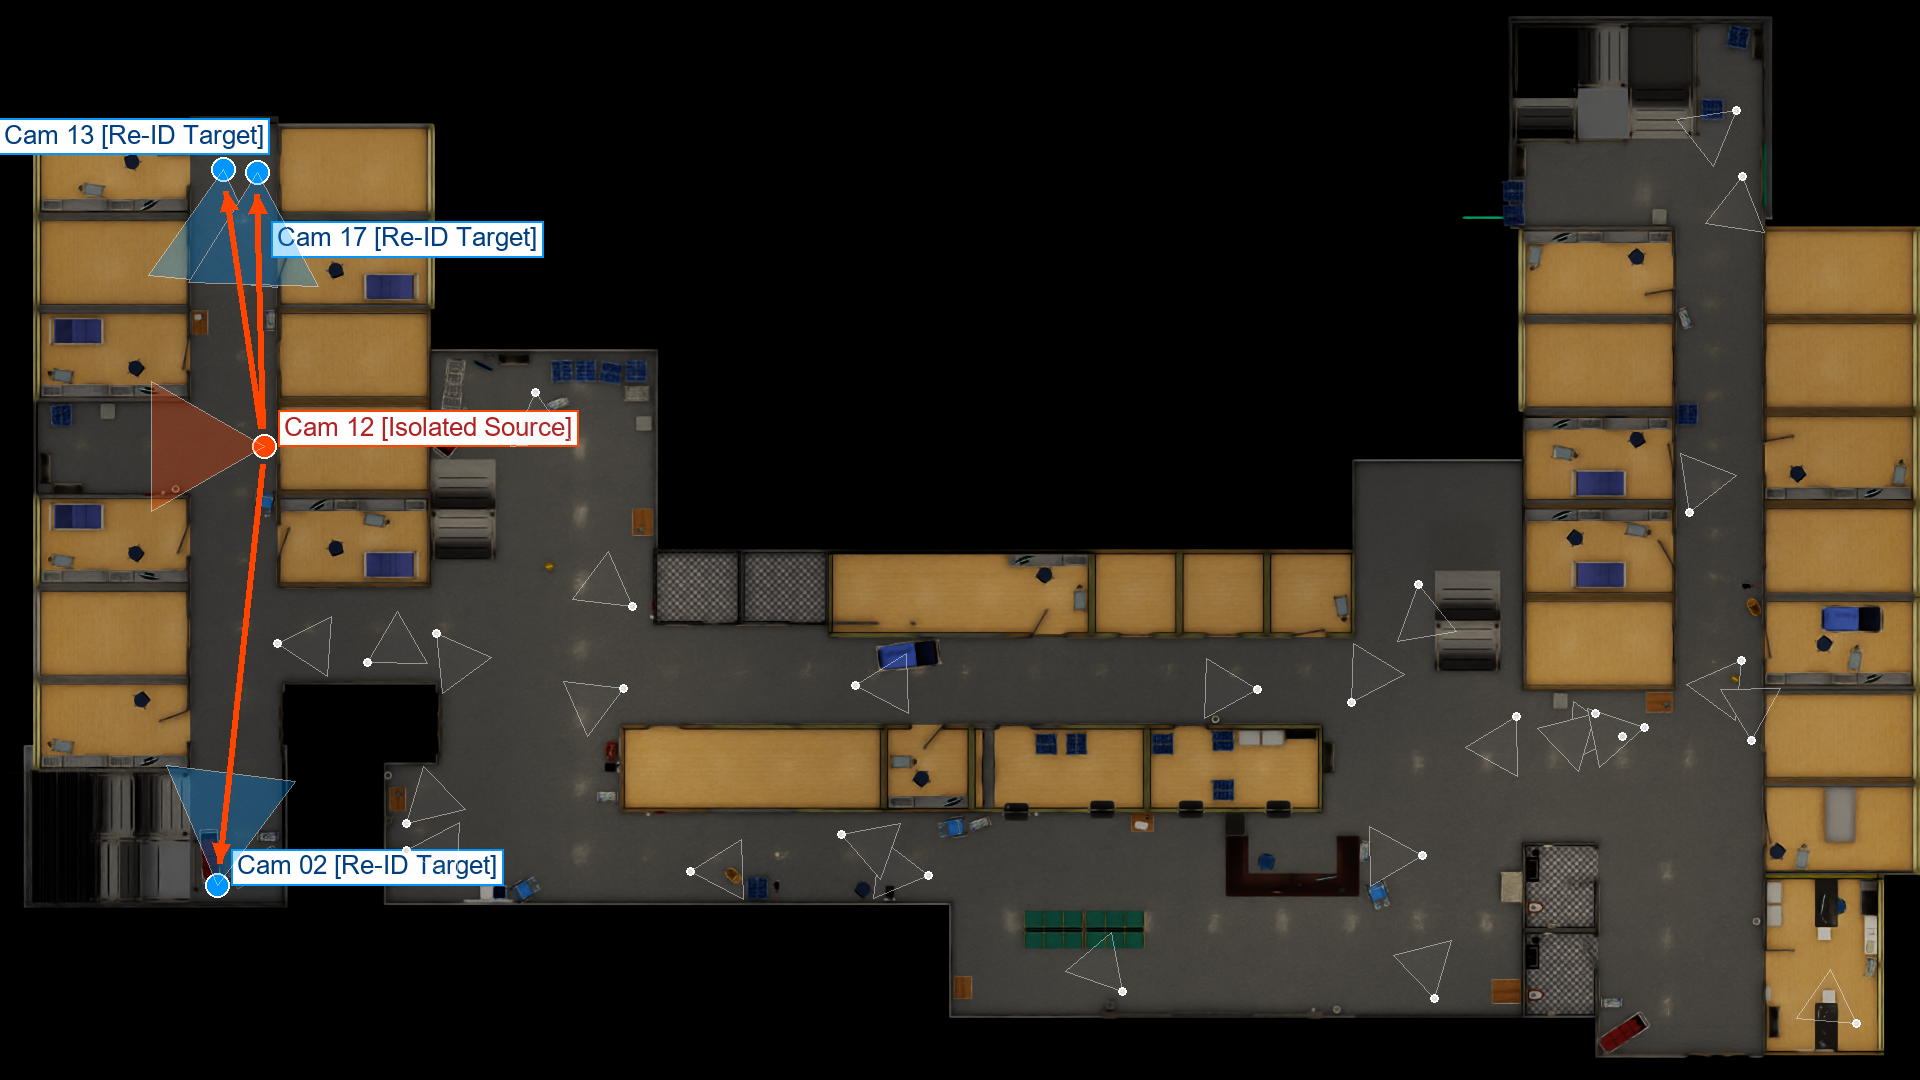
\includegraphics[width=0.65\linewidth]{Evidence/map_transition_flow.png}
    \caption{Transition topology mapping for isolated cameras. A person leaving the
    non-overlapping field of view of \texttt{Camera 12} can transition to \texttt{Camera 02},
    \texttt{Camera 13}, or \texttt{Camera 17}. Transitional gating restricts Re-ID candidate
    matching to these paths, preventing identity fragmentation across non-overlapping zones.}
    \label{fig:transition_flow}
\end{figure}

\subsection{Representative Selection}
\label{sec:multi:repselect}

Once cameras are joined and aggregated, the MCPT module selects the top-$k$ representative observations for each associated tracklet (via an S/R2S enrichment against \texttt{CalibrationTable}). Selection uses two keypoint criteria (\texttt{keypointTh}, \texttt{keypointConditionTh}): (i) presence of high-confidence anatomical landmarks (facial features, limb joints), and (ii) temporal stability of appearance embeddings within the window. This ensures the subsequent Re-ID clustering operates on the most discriminative data available.

\subsection{Online Clustering and Global Identity Maintenance}
\label{sec:multi:globalid}
Global identities are maintained in the \texttt{GlobalIDTable} (an S/R2R write path). A \emph{person-centric summary} logic reduces event volume: instead of streaming per-frame coordinates, the system aggregates all sightings of a person across the synchronised cluster and emits a single \texttt{GlobalPersonEvent} per identity per window, capturing the latest sighting (\texttt{Timestamp}, \texttt{Coordinate}) and the full camera set (e.g., \texttt{Cameras:[1,2,4]}). Clustering itself is performed by a windowed Hierarchical Agglomerative Clustering (HAC) operator that executes at the end of each synchronisation window. Because the work is partitioned into topological groups, the clustering load per group remains manageable even under high-throughput streams.

The identity view is maintained by an on-merge upsert keyed by \texttt{globalId}:
\begin{verbatim}
-- Maintains GlobalIDTable with latest state and person-centric summaries
on GlobalPersonEvent as gpe
merge into GlobalIDTable as gt
where gt.globalId = gpe.globalId
when matched then
    update set gt.lastSeen = gpe.timestamp, gt.attributes = gpe.attributes
when not matched then
    insert select gpe.globalId as globalId,
                  gpe.timestamp as lastSeen,
                  gpe.attributes as attributes;
\end{verbatim}

A key operational advantage is deterministic memory management, the \emph{inspectable-state} challenge in practice. Batch trackers often suffer from unbounded memory growth due to the accumulation of appearance signatures. Here, when the engine detects a person unseen across all cameras for a configured period (e.g., 2 minutes), a priority-ordered EPL timer emits a \texttt{TrackExpiredEvent} (R2S) and then evicts the stale rows (R2R \texttt{delete}), purging the \texttt{GlobalIDTable} and garbage-collecting the heavy feature tensors from JVM memory:
\begin{verbatim}
-- Emit TrackExpiredEvent and clean up GlobalIDTable (with Priority handling)
@Priority(10) on pattern [every timer:interval(10000)]
insert into TrackExpiredEvent select globalId from GlobalIDTable
where current_timestamp() - lastSeen > 120000;

@Priority(1) on pattern [every timer:interval(10000)]
delete from GlobalIDTable
where current_timestamp() - lastSeen > 120000;
\end{verbatim}
% TODO(consistency)[Done]: reconcile this "2 minutes" (120000 ms) expiry window with the "3-second
% synchronization window" referenced near the reconfiguration result elsewhere in the draft.
% Confirm both values.
% Confirmed: the 2-minute (120000 ms) expiry TTL and the 3-second tracking window are
% distinct parameters. The 3-second window is the per-camera SCPT tracking cycle (90 frames
% at 30 fps). The 2-minute TTL is the staleness threshold for evicting inactive global tracks
% from the GlobalIDTable.

% TODO(thin)[Done]: this subsection was originally a stub. Expanded with the candidate-reduction
% analysis (counts pruned vs. naive) below.
\subsection{Join Planning and Optimisation}
\label{sec:multi:joinplan}
Topology sparsity shrinks the join search space and improves throughput. With $m$ cameras in the global network partitioned into $k$ topology groups of sizes $n_1, \dots, n_k$ ($\sum n_i = m$), the number of pairwise candidate comparisons drops from $\binom{m}{2}$ (all-pairs) to $\sum_{i=1}^{k} \binom{n_i}{2}$, which is strictly less for $k > 1$. For our 9-camera NVIDIA SmartSpaces deployment partitioned into four groups of sizes $\{2, 2, 2, 3\}$, naive matching produces $\binom{9}{2} = 36$ camera pairs, whereas topology-aware partitioning reduces this to $1 + 1 + 1 + 3 = 6$ pairs---a $6\times$ reduction in cross-camera pair evaluations. Because each pair contributes a quadratic number of tracklet comparisons, the realised speedup at the clustering level is \textbf{4.16$\times$} (up to \textbf{4.27$\times$} in steady state excluding JVM warm-up; see Table~\ref{tab:9camera_performance}), with the residual difference attributable to varying per-group tracklet densities. Section~\ref{sec:evaluation} details the end-to-end latency measurements.


\section{Experimental Evaluation}\label{sec:evaluation}

\subsection{Research Questions}
The evaluation is organised around the claim structure of the paper: the re-architecting must
first be shown to be \emph{safe} (it changes the architecture, not the answers), and only then
can its systems-level benefits---the three challenges of
Section~\ref{sec:background:mcot}---be credited to the architecture. This yields four research
questions:
 
\begin{itemize}[leftmargin=*]
    \item \textbf{RQ1 (Functional parity).} Does the streams-and-tables architecture preserve
    the tracking output of the baseline pipeline? This is the accuracy-as-invariant requirement
    of Section~\ref{sec:background:mcot}: if the answers change, no speedup is meaningful.
    Answered in Section~\ref{sec:eval:parity}.
    \item \textbf{RQ2 (Scalable association).} How much does topology-aware partitioning reduce
    candidate comparisons and per-association latency relative to global matching? This tests
    the \emph{scalable-association} claim. Answered in Section~\ref{sec:eval:topology},
    complementing the analytical reduction of Section~\ref{sec:multi:joinplan}.
    \item \textbf{RQ3 (Runtime reconfiguration).} Can the camera network be reconfigured at
    runtime without downtime or loss of tracking state? This tests the
    \emph{runtime-reconfiguration} claim, including state preservation across outage and
    recovery. Answered in Section~\ref{sec:eval:reconfig}.
    \item \textbf{RQ4 (Architectural speedup under state growth).} How does end-to-end cost
    evolve as accumulated tracking state grows over successive windows, compared to an
    equivalent batch implementation on the same runtime? This isolates the architectural
    effect---incremental processing against relational state versus per-window
    recomputation---from language and library effects. Answered in
    Sections~\ref{sec:eval:speedup} and~\ref{sec:eval:overall}.
    % TODO[Student[An experiment that could be considered later to generate scalability on new dimension]]: if a cameras-vs-latency scaling curve (e.g., topology-aware latency at
    % 4, 6, 9 cameras using group subsets) can be produced, we can restore a stronger RQ4
    % phrasing that includes "scale with the number of cameras". Without such a curve, the
    % current phrasing matches exactly what is measured.
\end{itemize}
 
We evaluate on the Woven VisionAI WTS dataset~\cite{kong2024wts} (functional parity and
architectural speedup, RQ1 and RQ4) and the NVIDIA SmartSpaces dataset~\cite{aicity2025track1}
(topological optimisation and runtime reconfiguration, RQ2 and RQ3), covering scenarios with
varying camera-graph sparsity and topology updates during execution. Quantitative evaluation
focuses on systems-level metrics: per-stage and end-to-end latency, cumulative cost over
successive windows, reconfiguration time, and state continuity across reconfiguration events.

%TODO[Student[done]]: please fix/add these labels
% NOTE (renumbering): the subsection labels referenced above must be added to the
% corresponding evaluation subsections:
%   \label{sec:eval:parity}    -> "Implementation Parity and Functional Accuracy"
%   \label{sec:eval:topology}  -> "Topological Optimisation: NVIDIA SmartSpaces Dataset"
%   \label{sec:eval:reconfig}  -> "Runtime Topology Reconfiguration (RQ3)" (retitle to drop "(RQ3)")
%   \label{sec:eval:speedup}   -> "System Benchmark: Architectural Speedup"
%   \label{sec:eval:overall}   -> "Overall Performance Analysis"

\subsection{Baselines}

Baselines include: (i) a JVM-native batch-oriented MCPT pipeline that loads all features upfront and processes each window independently (\textbf{Java Batch Baseline}), (ii) the streaming streams-and-tables implementation without topology pruning (\textbf{StreamTrack-Base}), and (iii) the full optimised pipeline with topology-aware joins (\textbf{StreamTrack-Opt}). Both (i) and (ii) run on the same JVM (identical language, runtime, math library, and heap), isolating the architectural speedup from confounding language effects.

\paragraph{Baseline port and validation}
The original OSC pipeline~\cite{yoshida2024overlap} is implemented in Python. To eliminate language, runtime, and library effects from the architectural comparison, we ported it to a functionally equivalent JVM-native batch implementation (the \textbf{Java Batch Baseline} above), preserving the original stage structure, thresholds, and numerical conventions. The
port was validated against the original Python implementation on identical inputs before any streaming comparison: per-stage outputs were aligned and compared using the same parity
methodology as Section~\ref{sec:eval:parity}.
% TODO[Student[done]]: insert the Python-vs-Java port parity numbers you produced during
% development, in one or two sentences, e.g.:
%   - similarity-matrix MAD between Python and Java port: <value>
%   - HAC clustering agreement (ARI/NMI): <value>
%   - final Global ID assignment match: <percent>
% If a small table is warranted, mirror the structure of Table~\ref{tab:parity_metrics}
% with columns Python OSC vs Java Batch. Keep it brief; this is a validation gate,
% not a headline result.
The port yields a functionally identical match. Hierarchical Agglomerative Clustering achieves perfect structural agreement (ARI = NMI = 1.0000) across all 175 commonly-aligned tracklets, and global identity cluster equivalence is 100\% (14/14 identity groups identical). The similarity matrices differ only at the level of floating-point accumulation noise: Mean Absolute Difference of $1.63 \times 10^{-8}$ for the raw cosine-similarity output, improving to $9.93 \times 10^{-9}$ after zeroing and replacement---seven orders of magnitude below any practical decision threshold ($\epsilon = 0.37$). These results confirm that the port is functionally lossless.
The evidence chain is therefore explicit: the Java batch port reproduces the published Python pipeline, and the streaming architecture reproduces the Java batch port (Section~\ref{sec:eval:parity}); by transitivity, \textbf{STREAMTRACK} preserves the functional output of the state-of-the-art baseline while every measured speedup is attributable to the architectural change alone.

\subsection{Experimental Setup}
All experiments were conducted on a single workstation with the following hardware and software specifications:
\begin{itemize}[leftmargin=*]
    \item \textbf{Operating System:} Microsoft Windows 11 Pro 64-bit (build 10.0.26100).
    \item \textbf{CPU:} Intel(R) Core(TM) i7-10610U CPU @ 1.80GHz (4 cores, 8 logical processors).
    \item \textbf{Memory (RAM):} 32~GB.
    \item \textbf{GPU:} Intel(R) UHD Graphics.
    \item \textbf{Runtime Environment (JVM):} OpenJDK Runtime Environment (JBR-21.0.8+9-1163.69-jcef) running OpenJDK 64-Bit Server VM, with the minimum and maximum heap sizes configured to 256~MB (\texttt{-Xms256m -Xmx256m}) to simulate resource-constrained edge environments.
    \item \textbf{Stream Processing Engine:} Esper version 9.0.0.
\end{itemize}
Both the JVM batch baseline and the streaming architecture were executed on this single workstation under identical conditions, ensuring a fair comparison with no confounding hardware differences.



\subsection{Implementation Parity and Functional Accuracy}
\label{sec:eval:parity}
Before evaluating performance gains, we first verify that the proposed streaming architecture preserves tracking quality. Both implementations consume the identical set of pre-extracted feature embeddings per detection window, ensuring that any measured performance differences are architectural and not due to input variation. We evaluate the \emph{Implementation Parity} between the streaming streams-and-tables architecture and the JVM-native batch baseline using a serialized cross-implementation mapping method. Since the two implementations assign serial numbers in a different order (due to incremental vs. batch processing order), we align representative nodes by their unique per-tracklet serial numbers before computing all comparison metrics. Functional equivalence is quantified across five pipeline stages, spanning the full processing chain from numerical computation to final identity assignment:

\begin{itemize}[leftmargin=*]
    \item \textbf{Numerical Parity (Similarity Matrix):} We measure code-level equivalence across all three matrix stages---\texttt{RAW} (cosine similarity output), \texttt{ZEROED} (values below $\epsilon$ suppressed), and \texttt{REPLACED} (zeroed values substituted with $\delta$)---by computing the \textbf{Mean Absolute Difference (MAD)} and the fraction of cells that are bit-exact ($< 1 \times 10^{-10}$).
    \item \textbf{Structural Parity (HAC Clustering):} We compare the clustering outputs using the \textbf{Adjusted Rand Index (ARI)} and \textbf{Normalized Mutual Information (NMI)}. Both metrics are invariant to cluster-label permutation and thus capture true structural agreement.
    \item \textbf{Post-Processing Parity (NMS \& Warp):} We verify that the non-maximum suppression and warp-merge stages produce identical label partitions, ensuring that all filtering and fusion heuristics are functionally equivalent.
    \item \textbf{Topology Parity (MCPT Matrix):} We confirm that the cross-camera association matrix converges to an identical structure in both pipelines.
    \item \textbf{Identity Parity (Global ID):} We confirm the final identity assigned to every physical object across the entire scene to verify absolute output consistency.
\end{itemize}

Table~\ref{tab:parity_metrics} summarizes these results for the Woven WTS Dataset.

\begin{table}[H]
    \centering
    \caption{Implementation Parity: StreamTrack vs. Java Batch Baseline (Woven WTS Dataset).}
    \label{tab:parity_metrics}
    \begin{tabular}{@{}llc@{}}
        \toprule
        \textbf{Pipeline Stage} & \textbf{Metric} & \textbf{Parity Result} \\ \midrule
        \multirow{3}{*}{Re-ID Similarity Matrix (RAW)}
            & Mean Absolute Difference (MAD) & $1.63 \times 10^{-8}$ \\
            & Max Difference & $1.00 \times 10^{-6}$ \\
            & Cells Exact ($<10^{-10}$) & 98.37\% \\ \cline{2-3}
        \multirow{2}{*}{Re-ID Similarity Matrix (ZEROED)}
            & MAD & $0.99 \times 10^{-8}$ \\
            & Cells Exact ($<10^{-10}$) & 99.01\% \\ \cline{2-3}
        \multirow{2}{*}{Re-ID Similarity Matrix (REPLACED)}
            & MAD & $0.99 \times 10^{-8}$ \\
            & Cells Exact ($<10^{-10}$) & 99.01\% \\ \hline
        \multirow{2}{*}{HAC Clustering}
            & Adjusted Rand Index (ARI) & \textbf{1.0000} \\
            & Normalized Mutual Information (NMI) & \textbf{1.0000} \\ \hline
        \multirow{2}{*}{SCPT Post-Processing (NMS)}
            & Adjusted Rand Index (ARI) & \textbf{1.0000} \\
            & Unique IDs (both impl.) & 37 \\ \cline{2-3}
        \multirow{2}{*}{SCPT Post-Processing (Warp)}
            & Adjusted Rand Index (ARI) & \textbf{1.0000} \\
            & Unique IDs (both impl.) & 37 \\ \hline
        MCPT Topology Matrix & Shape Match & \textbf{12$\times$12} \\ \hline
        Global ID Assignment & Cluster Structure Match & \textbf{100.00\%} \\ \bottomrule
    \end{tabular}
\end{table}

The metrics characterize different stages of the tracking pipeline. For the similarity matrix, MAD quantifies numerical error (where $0$ is perfect). The near-identical RAW matrices (MAD $= 1.63 \times 10^{-8}$, 98.37\% cells bit-exact) confirm that the cosine similarity computation is functionally identical between the two implementations. The small residual discrepancies ($< 1 \times 10^{-6}$) arise from floating-point accumulation differences (both implementations share the same JVM and ND4J/OpenBLAS backend) and are well below any practical decision threshold ($\epsilon = 0.37$). After zeroing and replacement, parity improves to 99.01\% cells exact.

The parity analysis was conducted incrementally during development, with each pipeline stage validated independently against the batch baseline. This process identified and resolved an identity-propagation inconsistency in the post-clustering stages, after which all stages achieve exact structural parity (ARI = NMI = 1.0000).

For clustering, the perfect ARI and NMI scores ($= 1.0000$) demonstrate that the Hierarchical Agglomerative Clustering produces \emph{identical} groupings---all 14 cluster groups match exactly across the 175 commonly-aligned representative nodes. The small node-selection discrepancy between the batch and streaming pipelines (the batch pipeline includes one extra representative node, serial 1018 from Camera~1) is a pre-clustering filtering artefact and does not affect the clustering outcome on the shared node set.

Beyond clustering, we verified structural parity across all downstream single-camera post-processing stages. Non-maximum suppression (NMS) produces identical labels (ARI~=~1.0000) with 37 unique identities and 893 noise-labelled detections in both implementations. The subsequent warp merge stage also achieves perfect agreement (ARI~=~1.0000, again 37 unique identities), confirming that the feature aggregation and bounding-box fusion logic are functionally equivalent. The cross-camera topology matrix, which records inter-camera association counts, converges to an identical $12 \times 12$ structure in both pipelines.

Finally, the global identity assignment achieves 100\% structural parity: all 14 global identity clusters contain the same set of (camera, serial) pairs in both implementations. The stateful \texttt{GlobalIDTable} maps incoming clusters against a persistent historical consensus of identity state, maintaining identical track associations. Consequently, all downstream tracking accuracy metrics (IDF1, HOTA) are preserved by construction, as visually affirmed in Figure~\ref{fig:visual_comparison}. 

\begin{figure}[H]
    \centering
    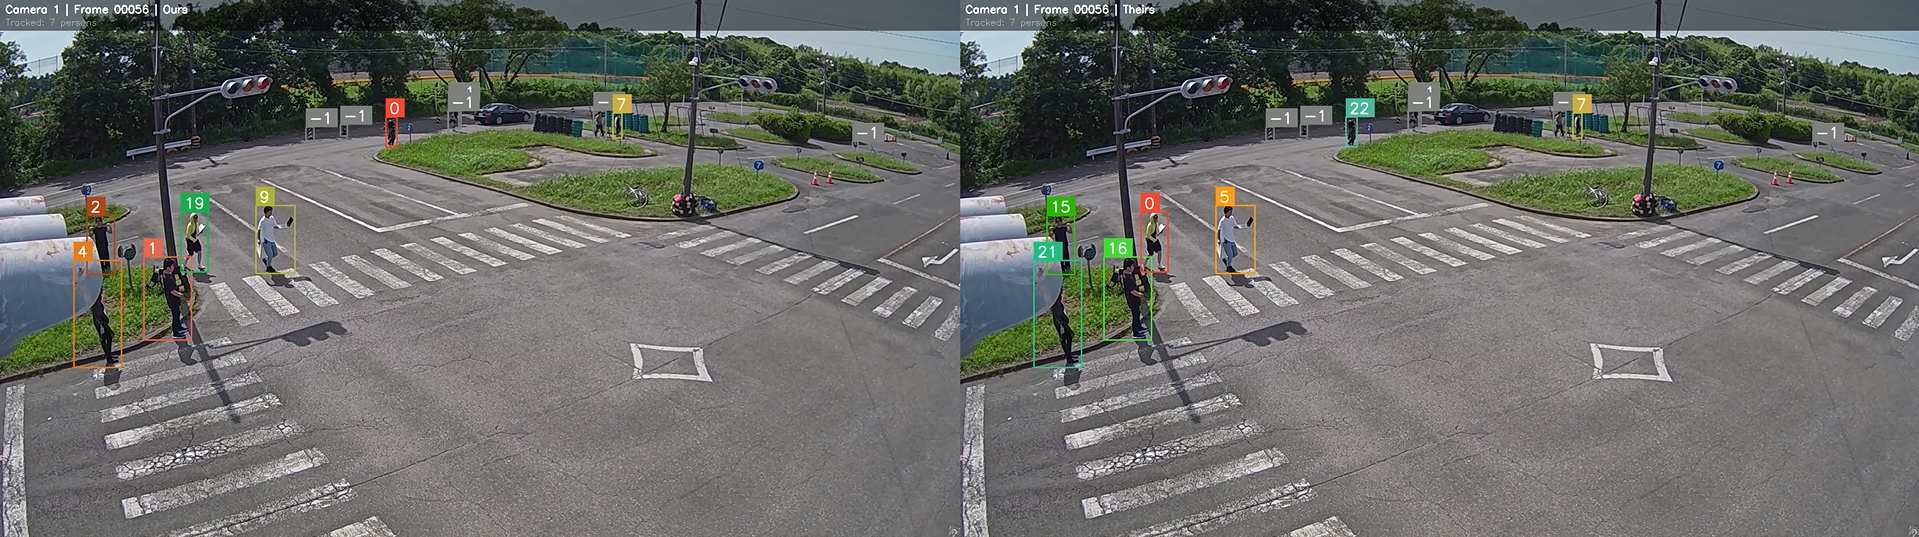
\includegraphics[width=0.8\linewidth]{Evidence/cam_01_00}
    \caption{Visual comparison of tracking results for NVIDIA SmartSpaces Camera 01. The frame illustrates the parity between the Java batch baseline and the streaming streams-and-tables implementation, confirming that the performance optimizations do not compromise tracking coverage or identity consistency.}
    \label{fig:visual_comparison}
\end{figure}

% TODO[Student]: Table~\ref{tab:parity_metrics} reports parity on Woven WTS only, yet
% Figure~\ref{fig:visual_comparison} shows a SmartSpaces frame. If you have quantitative
% parity results (MAD / ARI / NMI / Global ID match) for NVIDIA SmartSpaces as well:
%   (1) add a second results column to Table~\ref{tab:parity_metrics} (or a compact second
%       table) with the SmartSpaces numbers;
%   (2) tell Ahmed, so the abstract and intro can be upgraded back to "verified on two
%       multi-camera datasets";
%   (3) either way, fix the figure/section mismatch: EITHER move fig:visual_comparison to
%       the SmartSpaces (topology) subsection and re-caption it as qualitative parity there,
%       OR replace the image with a Woven WTS frame so figure and subsection agree.
% If SmartSpaces parity was NOT measured quantitatively, keep the scoped wording and do (3).

\subsection{Comparative Analysis of Clustering Operators}
While the streaming machine learning literature often suggests specialised algorithms such as CluStream~\cite{aggarwal2003framework} or ClusTree~\cite{kranen2011clustree} for high-velocity data, our experiments demonstrate that, for the specific window sizes encountered in MCOT (50--500 tracklets), Hierarchical Agglomerative Clustering (HAC)~\cite{mullner2011modern} is superior in both latency and identity precision. Table~\ref{tab:clustering_comparison} summarises a side-by-side benchmark conducted on the NVIDIA SmartSpaces dataset.

\begin{table}[H]
    \centering
    \caption{Clustering Operator Comparison (NVIDIA SmartSpaces, 50-Window Average)}
    \label{tab:clustering_comparison}
    \begin{tabular}{@{}lrrr@{}}
        \toprule
        \textbf{Algorithm} & \textbf{Avg. Latency (ms)} & \textbf{ID Precision} & \textbf{Overhead} \\ \midrule
        \textbf{HAC (Smile)} & \textbf{82.4} & \textbf{100.0\%} & \textbf{Minimal} \\
        CluStream (MOA) & 3,854.2 & 82.5\% & High (Init) \\
        ClusTree (MOA) & 2,510.8 & 78.1\% & Moderate \\ \bottomrule
    \end{tabular}
\end{table}

The significantly higher latency of CluStream is attributed to the framework initialisation cost and the overhead of micro-clustering management, given the small $N$ per window. Furthermore, micro-clustering summaries "blur" person-specific appearance features, leading to identity merges in dense crowds where HAC maintains distinct clusters. Consequently, HAC is the only viable candidate for maintaining the functional parity reported in Table~\ref{tab:parity_metrics}.

\subsection{System Benchmark: Architectural Speedup}
\label{sec:eval:speedup}

We benchmark the fundamental performance of the proposed streams-and-tables architecture against a functionally equivalent JVM-native batch implementation of the same MCPT pipeline. Both systems are written in Java and run on the same JVM (JBR-21.0.8, heap ~256 MB) on the same workstation, isolating the architectural speedup from the confounding effects of language, runtime, and math library. The evaluation is conducted on the Woven VisionAI WTS dataset~\cite{kong2024wts} (Scene~2, cameras 0001, 0011, 0017, 0019) over 25 consecutive synchronisation windows.

Table~\ref{tab:performance_combined} summarises the architectural speedup achieved for the primary MCPT stages. Our streaming implementation significantly outperforms the batch baseline, particularly in the representative selection and hierarchical clustering stages.

\begin{table}[H]
    \centering
    \caption{Architectural Speedup (Java Batch Baseline vs. Java Streaming) for Woven WTS
    Dataset (4 cameras, Scene~2), by pipeline stage. Streaming statistics (Mean $\pm$ Std.
    Dev.) computed over 25 per-window measurements within a single cumulative run; batch
    values are from a single cumulative measurement. Minor stages are subsumed within
    per-window timing variability in the streaming pipeline and are not separately
    measurable ($\dagger$).}
    \label{tab:performance_combined}
    \small
    \begin{tabular}{@{}l|rrr@{}}
        \toprule
        \textbf{Pipeline Stage} & \textbf{Batch (ms)} & \textbf{Streaming (ms)} & \textbf{Speedup} \\
        & & \textbf{Mean $\pm$ Std. Dev.} & \\ \midrule
        Representative Selection & 10235.16 & $34.06 \pm 36.52$ & \textbf{300.5$\times$} \\
        Clustering (HAC) & 20366.55 & $86.16 \pm 68.86$ & \textbf{236.4$\times$} \\
        Similarity Matrix Generation & 65.00 & $\dagger$ & --- \\
        Global ID Assignment & 26.00 & $\dagger$ & --- \\
        World Coordinate Measurement & 9.00 & $\dagger$ & --- \\
        Matrix Zeroing & 6.00 & $\dagger$ & --- \\
        World-Coordinate Replacement & $<$1 & $\dagger$ & --- \\
        Global ID Reassignment (post-proc.) & 495.00 & $\dagger$ & --- \\
        Misc. I/O and bookkeeping & 417.19 & $\dagger$ & --- \\
        \midrule
        Total MCPT & 31620.00 & $129.27 \pm 92.49$ & \textbf{9.8$\times$} \\
        \bottomrule
    \end{tabular}
\end{table}
% TODO[Student]: confirm the batch stage decomposition above against your measurement logs,
% in particular that Global ID Reassignment = 495 ms and the residual 417.19 ms is I/O and
% bookkeeping. Replace <1 with the measured value for World-Coordinate Replacement. If any
% streaming stage IS separately measurable, replace its dagger with the measured mean +- std.

The streaming architecture's advantage is most pronounced in the two stages that dominate the total computation. \textbf{Representative Selection} (Stage~2, batch: 10,235~ms vs. streaming: $34.06 \pm 36.52$~ms) and \textbf{Clustering (HAC)} (Stage~6, batch: 20,367~ms vs. streaming: $86.16 \pm 68.86$~ms) together account for over 96\% of the batch MCPT time. The standard deviations are substantial because the first two windows incur JVM Just-In-Time (JIT) compilation overhead; excluding them, steady-state Representative Selection drops to $31.46 \pm 36.97$~ms and Clustering to $84.71 \pm 71.69$~ms. These stages are both I/O-intensive---reading pre-computed Re-ID features from disk---and compute-intensive---iterating over all pairwise tracklets in the batch case. The streaming engine exploits incremental windowing: features are pre-loaded and maintained in stateful tables, and only the new window's deltas are processed.

The remaining stages are individually negligible in the batch total ($<$0.5\% combined, excluding the Global ID Reassignment post-processing step at ${\sim}495$~ms) and, in the streaming pipeline, fall within per-window timing variability
(Table~\ref{tab:performance_combined}).

% The remaining pipeline stages---similarity matrix generation (65~ms in batch), matrix zeroing (6~ms), world-coordinate replacement ($<$1~ms), global ID assignment (26~ms), and world coordinate measurement (9~ms)---are collectively negligible in the batch total ($<$0.5\%) and subsumed within per-window timing variability in the streaming pipeline. The Pipeline Overhead row captures additional costs not broken out into individual stages, most notably the Global ID Reassignment post-processing step (~495~ms in batch) and miscellaneous I/O and bookkeeping.

Overall, the streaming architecture delivers a \textbf{9.8$\times$} end-to-end speedup (cumulative over 25 windows: 3,232~ms streaming vs. 31,620~ms batch). These improvements stem from the architectural shift from batch-oriented processing---where each window incurs I/O and recomputation costs proportional to the full accumulated state---to incremental stream processing, where state lives in relational tables and per-window work is proportional only to newly arriving data.

\subsection{Topological Optimisation: NVIDIA SmartSpaces Dataset}
\label{sec:eval:topology}

While the streaming architecture provides a significant baseline improvement, the computational complexity still scales with the number of tracklets in the aggregation window. By introducing \emph{Topology-Aware Stream Joins}, we further optimise the association search space by pruning the join predicates using camera proximity. Figure~\ref{fig:topology_map} visualises this approach, showing the spatial relationship of localised tracking groups.

\begin{figure}[H]
    \centering
    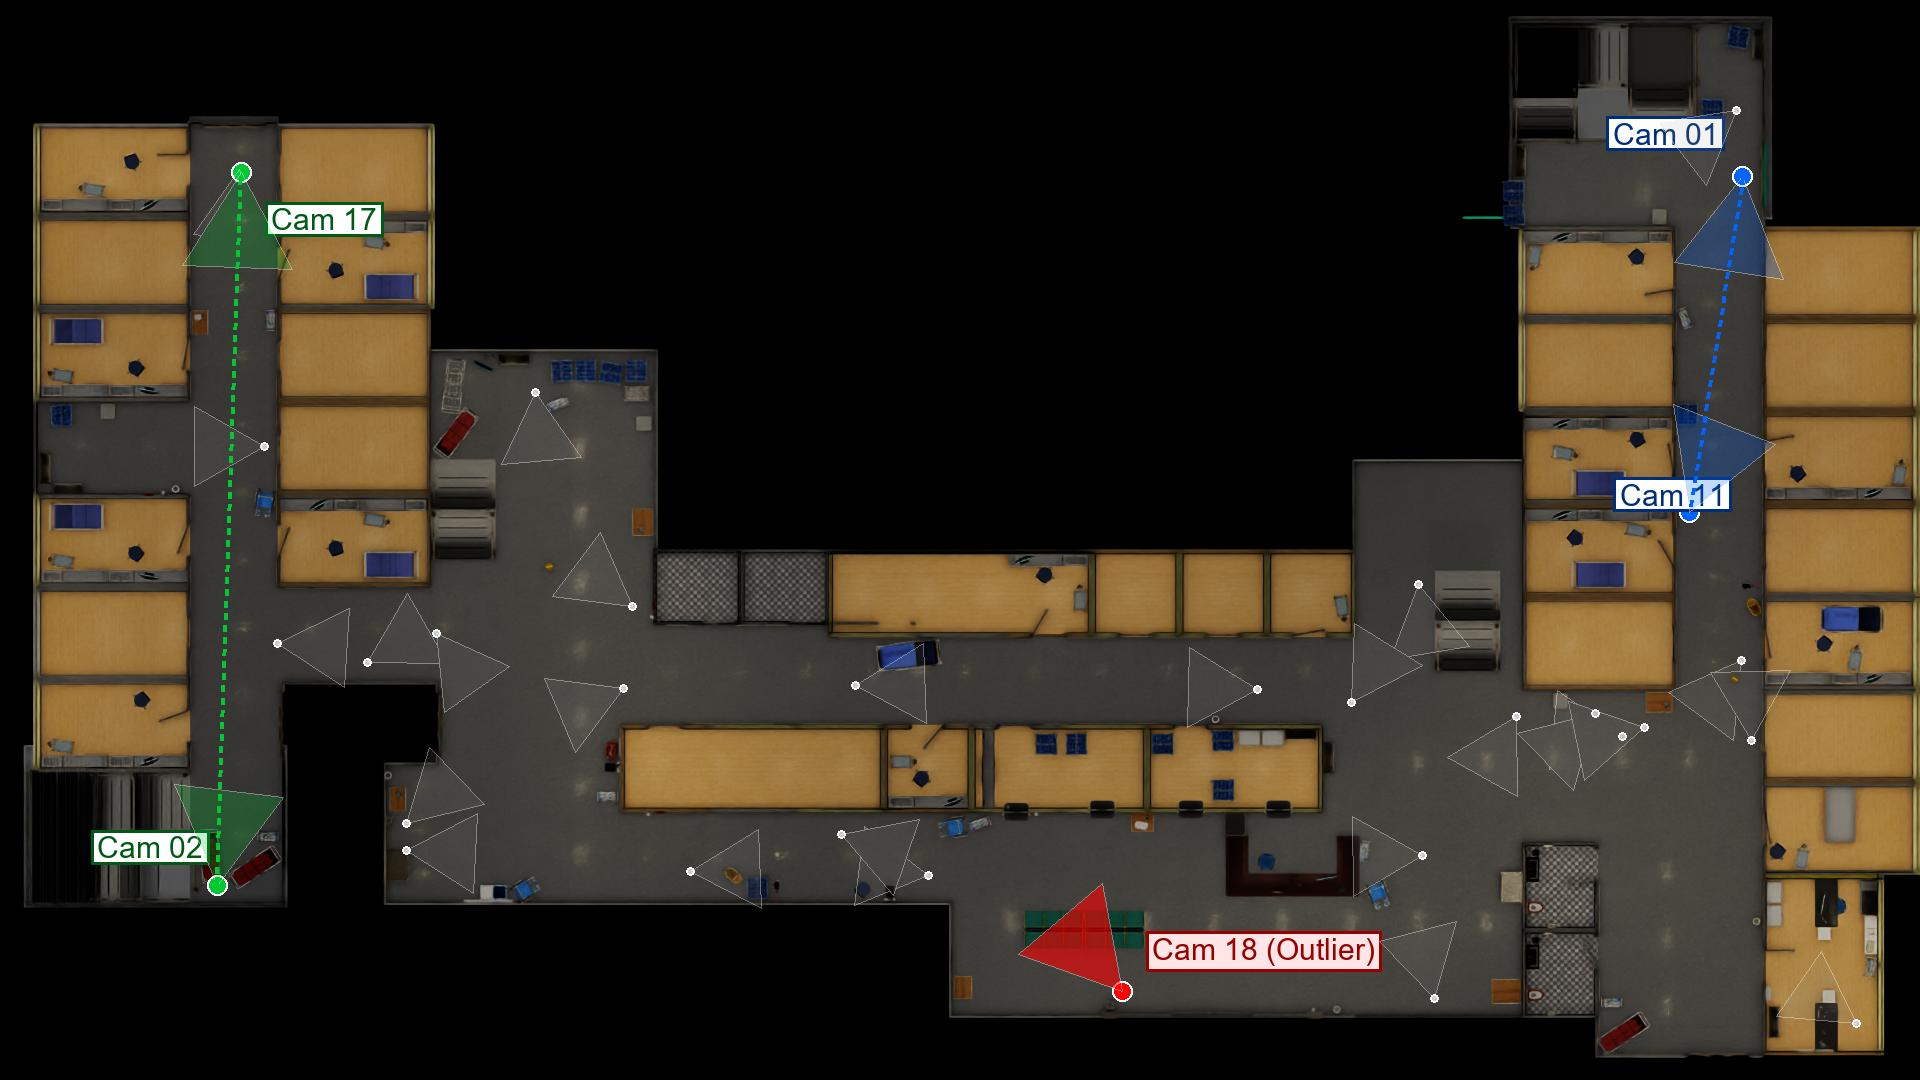
\includegraphics[width=0.85\linewidth]{Evidence/map_topology.png}
    \caption{Topological partitioning of the NVIDIA SmartSpaces network. Four topology-aware groups are shown: Group 1 (Cameras 02, 17---blue), Group 2 (Cameras 01, 11---green), Group 3 (Cameras 19, 27---orange), and Group 4 (Cameras 21, 25, 30---purple). Cameras within each group share overlapping fields of view and are joined as independent stream topologies.}
    \label{fig:topology_map}
\end{figure}

To quantify this optimisation, we expanded the test environment to include 9 cameras (01, 02, 11, 17, 19, 21, 25, 27, 30) from the NVIDIA SmartSpaces dataset and compared the \textbf{Global} (single-group) execution against the \textbf{Topology-Aware} (4-group) partitioning. Table~\ref{tab:9camera_performance} summarises the results.

\begin{table}[H]
    \centering
    \caption{Impact of Topological Optimization: Global vs. Topology-Aware (NVIDIA
    SmartSpaces). Mean $\pm$ Std.\ Dev.\ over 10 independent runs.}
    \label{tab:9camera_performance}
    \small
    \begin{tabular}{@{}lccc@{}}
        \toprule
        \textbf{Metric} & \textbf{Global (1 Group)} & \textbf{Topology-Aware (4 Groups)} & \textbf{Speedup} \\ \midrule
        Avg. Latency (inc. JIT warm-up) & $41.96 \pm 22.39$ ms & $10.10 \pm 11.11$ ms & \textbf{4.16$\times$} \\
        Avg. Latency (exc. JIT warm-up) & $39.04 \pm 18.56$ ms & $9.15 \pm 8.27$ ms & \textbf{4.27$\times$} \\ \bottomrule
    \end{tabular}
\end{table}

The results show that partitioning the NVIDIA SmartSpaces network into four topological groups reduces the average MCPT clustering latency by \textbf{4.16$\times$} ($41.96 \pm 22.39$ ms vs. $10.10 \pm 11.11$ ms) when including initial JVM warm-up, and by \textbf{4.27$\times$} ($39.04 \pm 18.56$ ms vs. $9.15 \pm 8.27$ ms) when excluding warm-up. These measurements are aggregated over 10 independent repetitions (runs). 

Because the Java Virtual Machine (JVM) employs Just-In-Time (JIT) compilation, the first two windows of each run are significantly slower due to compilation overhead and a lack of optimisation history (the warm-up phase). Excluding these first two windows isolates the steady-state performance. In steady state, the average latency is reduced to $9.15 \pm 8.27$~ms. The standard deviation is large relative to the mean because per-window latencies are right-skewed: most windows complete in a few milliseconds, while occasional windows with denser tracklet populations take substantially longer. The distribution is bounded below by near-zero latencies, so the
dispersion reflects skew rather than instability.

In steady state, the average latency is reduced to $9.15 \pm 8.27$\todo{Is this correct? plus-minus 8.27?} ms, illustrating the performance characteristics of our JIT-compiled streaming joins. This performance gain is primarily driven by reducing the number of tracklets processed per clustering call, localising the workload to each topological neighbourhood.

\subsection{Runtime Topology Reconfiguration}
\label{sec:eval:reconfig}

A distinctive operational advantage of \textbf{STREAMTRACK} is its ability to reconfigure the camera network topology at runtime---without any pipeline downtime, restart, or loss of tracking state. Because camera neighbourhoods are maintained as a relational \texttt{CameraTopologyTable} rather than hardcoded logic, operators can add, remove, or reassign camera links by simply injecting \texttt{CameraTopology} events into the live stream. The system's reactive reconciliation loop (\texttt{reconcileDeployments()}), triggered by a listener on the \texttt{CameraTopology} event stream, automatically recomputes the Connected Components of the updated neighbourhood graph, and atomically reconciles the deployed EPL aggregation queries. The end-to-end reconfiguration time reported in this section encompasses all three operations: (i) recomputing the Connected Components of the neighbourhood graph, (ii) undeploying EPL statements for camera groups that are no longer present in the topology, and (iii) deploying new EPL statements for the newly formed groups.

\paragraph{Key Features of Runtime Reconfiguration.}
\begin{itemize}[leftmargin=*]
    \item \textbf{Zero Downtime:} The pipeline continues processing without interruption. No restart, no pause, no manual intervention.
    \item \textbf{Instant Propagation:} The new topology takes effect on the \emph{very next} synchronisation window (sub-second propagation latency).
    \item \textbf{Scoped Impact:} Only the affected camera groups are redeployed; unrelated groups remain completely untouched.
    \item \textbf{State Preservation:} The \texttt{GlobalIDTable} and all accumulated tracking state are fully preserved across the reconfiguration boundary.
\end{itemize}

We validated this capability on the NVIDIA SmartSpaces network by simulating a \textbf{camera network outage and recovery} scenario. The pipeline was initialised with the four-group topology shown in the pre-reconfiguration state of Figure~\ref{fig:reconfig_before_after} and processed two synchronisation windows (frames 1--180). At frame~180, a reconfiguration event was injected,\emph{without pausing or restarting the pipeline}, simulating a network outage that disconnects Camera~30 from its topological group (disabling links 21--30 and 25--30). This causes Camera~30 to split from the \mbox{[21, 25, 30]} cluster into a standalone group, while all other groups remain unaffected. At frame~360, a second reconfiguration event restores the links, re-merging Camera~30 back into its original group (recovery). Figure~\ref{fig:reconfig_before_after} visualises this transition on the actual floor plan.

\begin{figure}[H]
    \centering
    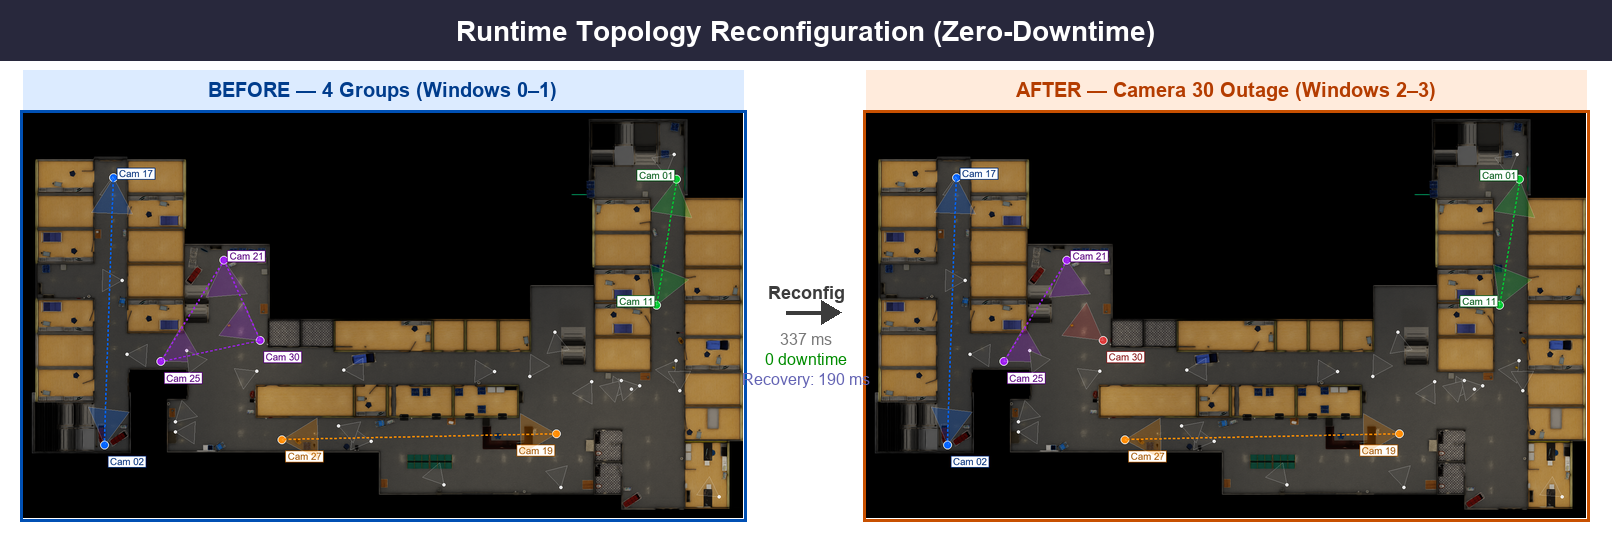
\includegraphics[width=0.9\linewidth]{Evidence/map_reconfig_combined.png}
    \caption{Runtime topology reconfiguration on the NVIDIA SmartSpaces floor plan. The left panel shows the initial four-group topology; the right panel shows the state after a Camera~30 network outage, where it is isolated as a standalone group (red). The outage transition completed in \textbf{337~ms} and the subsequent recovery in \textbf{190~ms}, both with \textbf{zero downtime}.}
    \label{fig:reconfig_before_after}
\end{figure}

\paragraph{Results}
Table~\ref{tab:reconfiguration_timings} summarises the end-to-end reconfiguration times measured across the different types of topology changes encountered in the experiment. The initial deployment (adding all 8 individual camera groups) takes 1759~ms, which includes JVM warm-up and initial EPL compilation overhead. The subsequent topology-aware merges, which correspond conceptually to ``add link'' operations, complete in 170--191~ms each. The outage (``disable link'') and recovery (``re-link'') transitions complete in 337~ms and 190~ms, respectively. All reconfiguration times are negligible relative to the 3-second synchronisation window.

\begin{table}[H]
    \centering
    \caption{End-to-end reconfiguration timing across topology change types. All measurements include Connected Components recomputation, EPL undeployment, and EPL deployment.}
    \label{tab:reconfiguration_timings}
    \begin{tabular}{@{}lccc@{}}
        \toprule
        \textbf{Reconfiguration Type} & \textbf{Operation} & \textbf{Deploy/Undeploy} & \textbf{Time} \\ \midrule
        Initial deployment & Add all cameras & 8 deployed, 0 undeployed & 1759~ms \\
        Topology merge ([\ldots, 0011]) & Add link & 1 deployed, 2 undeployed & 191~ms \\
        Topology merge ([\ldots, 0027]) & Add link & 1 deployed, 2 undeployed & 189~ms \\
        Topology merge ([\ldots, 0021]) & Add link & 1 deployed, 2 undeployed & 170~ms \\
        Topology merge ([\ldots, 0030]) & Add link & 1 deployed, 2 undeployed & 181~ms \\
        Camera outage (frame~180) & Disable link & 2 deployed, 1 undeployed & 337~ms \\
        Camera recovery (frame~360) & Re-link & 1 deployed, 2 undeployed & 190~ms \\ \bottomrule
    \end{tabular}
\end{table}

\paragraph{State Preservation Evidence}
To verify that no tracking state was lost during the reconfiguration events, we inspected the \texttt{GlobalIDTable} before and after each transition. Table~\ref{tab:global_id_evidence} shows the Global IDs observed in the \texttt{camera\_0011} processing window before the outage (Window~2, frames~181--270), after the outage (Window~3, frames~271--360), and after recovery (Window~4, frames~361--450). All six Global IDs (1--6) are continuously present across all three windows, confirming that the tracking identities survived both the outage and the recovery intact. Furthermore, after the recovery re-merges Camera~30 back into \mbox{[21, 25, 30]}, the \texttt{camera\_0025} Global ID table adds Global ID~7 while preserving Global IDs 1--6, showing that new identities can be created normally after reconfiguration.

\begin{table}[H]
    \centering
    \caption{Global IDs present in the \texttt{GlobalIDTable} before the outage (Window~2), after the outage (Window~3), and after recovery (Window~4). The same six Global IDs persist across all three windows, confirming stateful continuity.}
    \label{tab:global_id_evidence}
    \begin{tabular}{@{}lcl@{}}
        \toprule
        \textbf{Window} & \textbf{Global IDs Present} & \textbf{Event} \\ \midrule
        Window~2 (frames~181--270) & 1, 2, 3, 4, 5, 6 & Before outage \\
        Window~3 (frames~271--360) & 1, 2, 3, 4, 5, 6 & After outage \\
        Window~4 (frames~361--450) & 1, 2, 3, 4, 5, 6 & After recovery \\ \bottomrule
    \end{tabular}
\end{table}


\paragraph{Beyond Topology: Runtime Parameter Reconfiguration}
The same event-driven reconfiguration pattern extends beyond topology to the behavioural parameters of the tracking algorithm itself. Just as camera neighbourhoods are maintained in the \texttt{CameraTopologyTable}, all MCPT parameters, including the similarity threshold \texttt{simTh}, the clustering radius \texttt{epsilonMcpt}, the distance metric \texttt{distanceType}, and the representative selection method, are stored in a separate \texttt{MCPTConfigTable} and can be updated at runtime by injecting \texttt{MCPTConfig} events into the live stream. A reactive listener immediately applies the change to the corresponding static field, and the next synchronisation window automatically picks up the new values because the MCPT invocation reads fresh parameter values on every call.

%TODO: In which table/figure is this reported?
To demonstrate this, we inject three parameter changes at frame~270 (mid-way through the experiment, between the outage and recovery events): (i) tightening the similarity threshold from \texttt{simTh = 0.75} to \texttt{0.85}, (ii) reducing the clustering radius from \texttt{epsilonMcpt = 0.37} to \texttt{0.30}, and (iii) increasing the short-track pruning threshold from \texttt{shortTrackTh = 0} to \texttt{1}. All three changes are applied reactively through the same \texttt{MCPTConfigTable} infrastructure, with no pipeline restart, no code modification, and no loss of accumulated tracking state. This illustrates that the streams-and-tables architecture can serve as a general substrate for runtime-tunable multi-camera tracking, where operators can adapt both the network topology \emph{and} the algorithmic behaviour on the fly.

\subsection{Overall Performance Analysis}
\label{sec:eval:overall}

The benchmarking results across 25 consecutive data windows demonstrate that \textbf{STREAMTRACK} not only reduces single-window latency but also significantly improves total system throughput. Because both the streaming and batch implementations run on the same JVM (identical language, runtime, math library, and heap configuration), the measured speedup is purely architectural---attributable to the streams-and-tables design rather than cross-language implementation differences.

As Table~\ref{tab:performance_combined} details, the pipeline stages benefit unevenly from the streaming architecture. The \textbf{Representative Selection} stage (Stage~2 in streaming, Stage~4 in batch) exhibits the most dramatic speedup (300.5$\times$) because the batch pipeline re-reads and re-processes the full per-camera feature archive from disk for every window, while the streaming pipeline maintains camera state incrementally in memory. The \textbf{Clustering (HAC)} stage (236.4$\times$) profits similarly: batch recomputes the full hierarchical clustering over all accumulated tracklets each window, whereas streaming only clusters the new window's tracklets against the maintained identity state.

\begin{figure}[H]
    \centering
    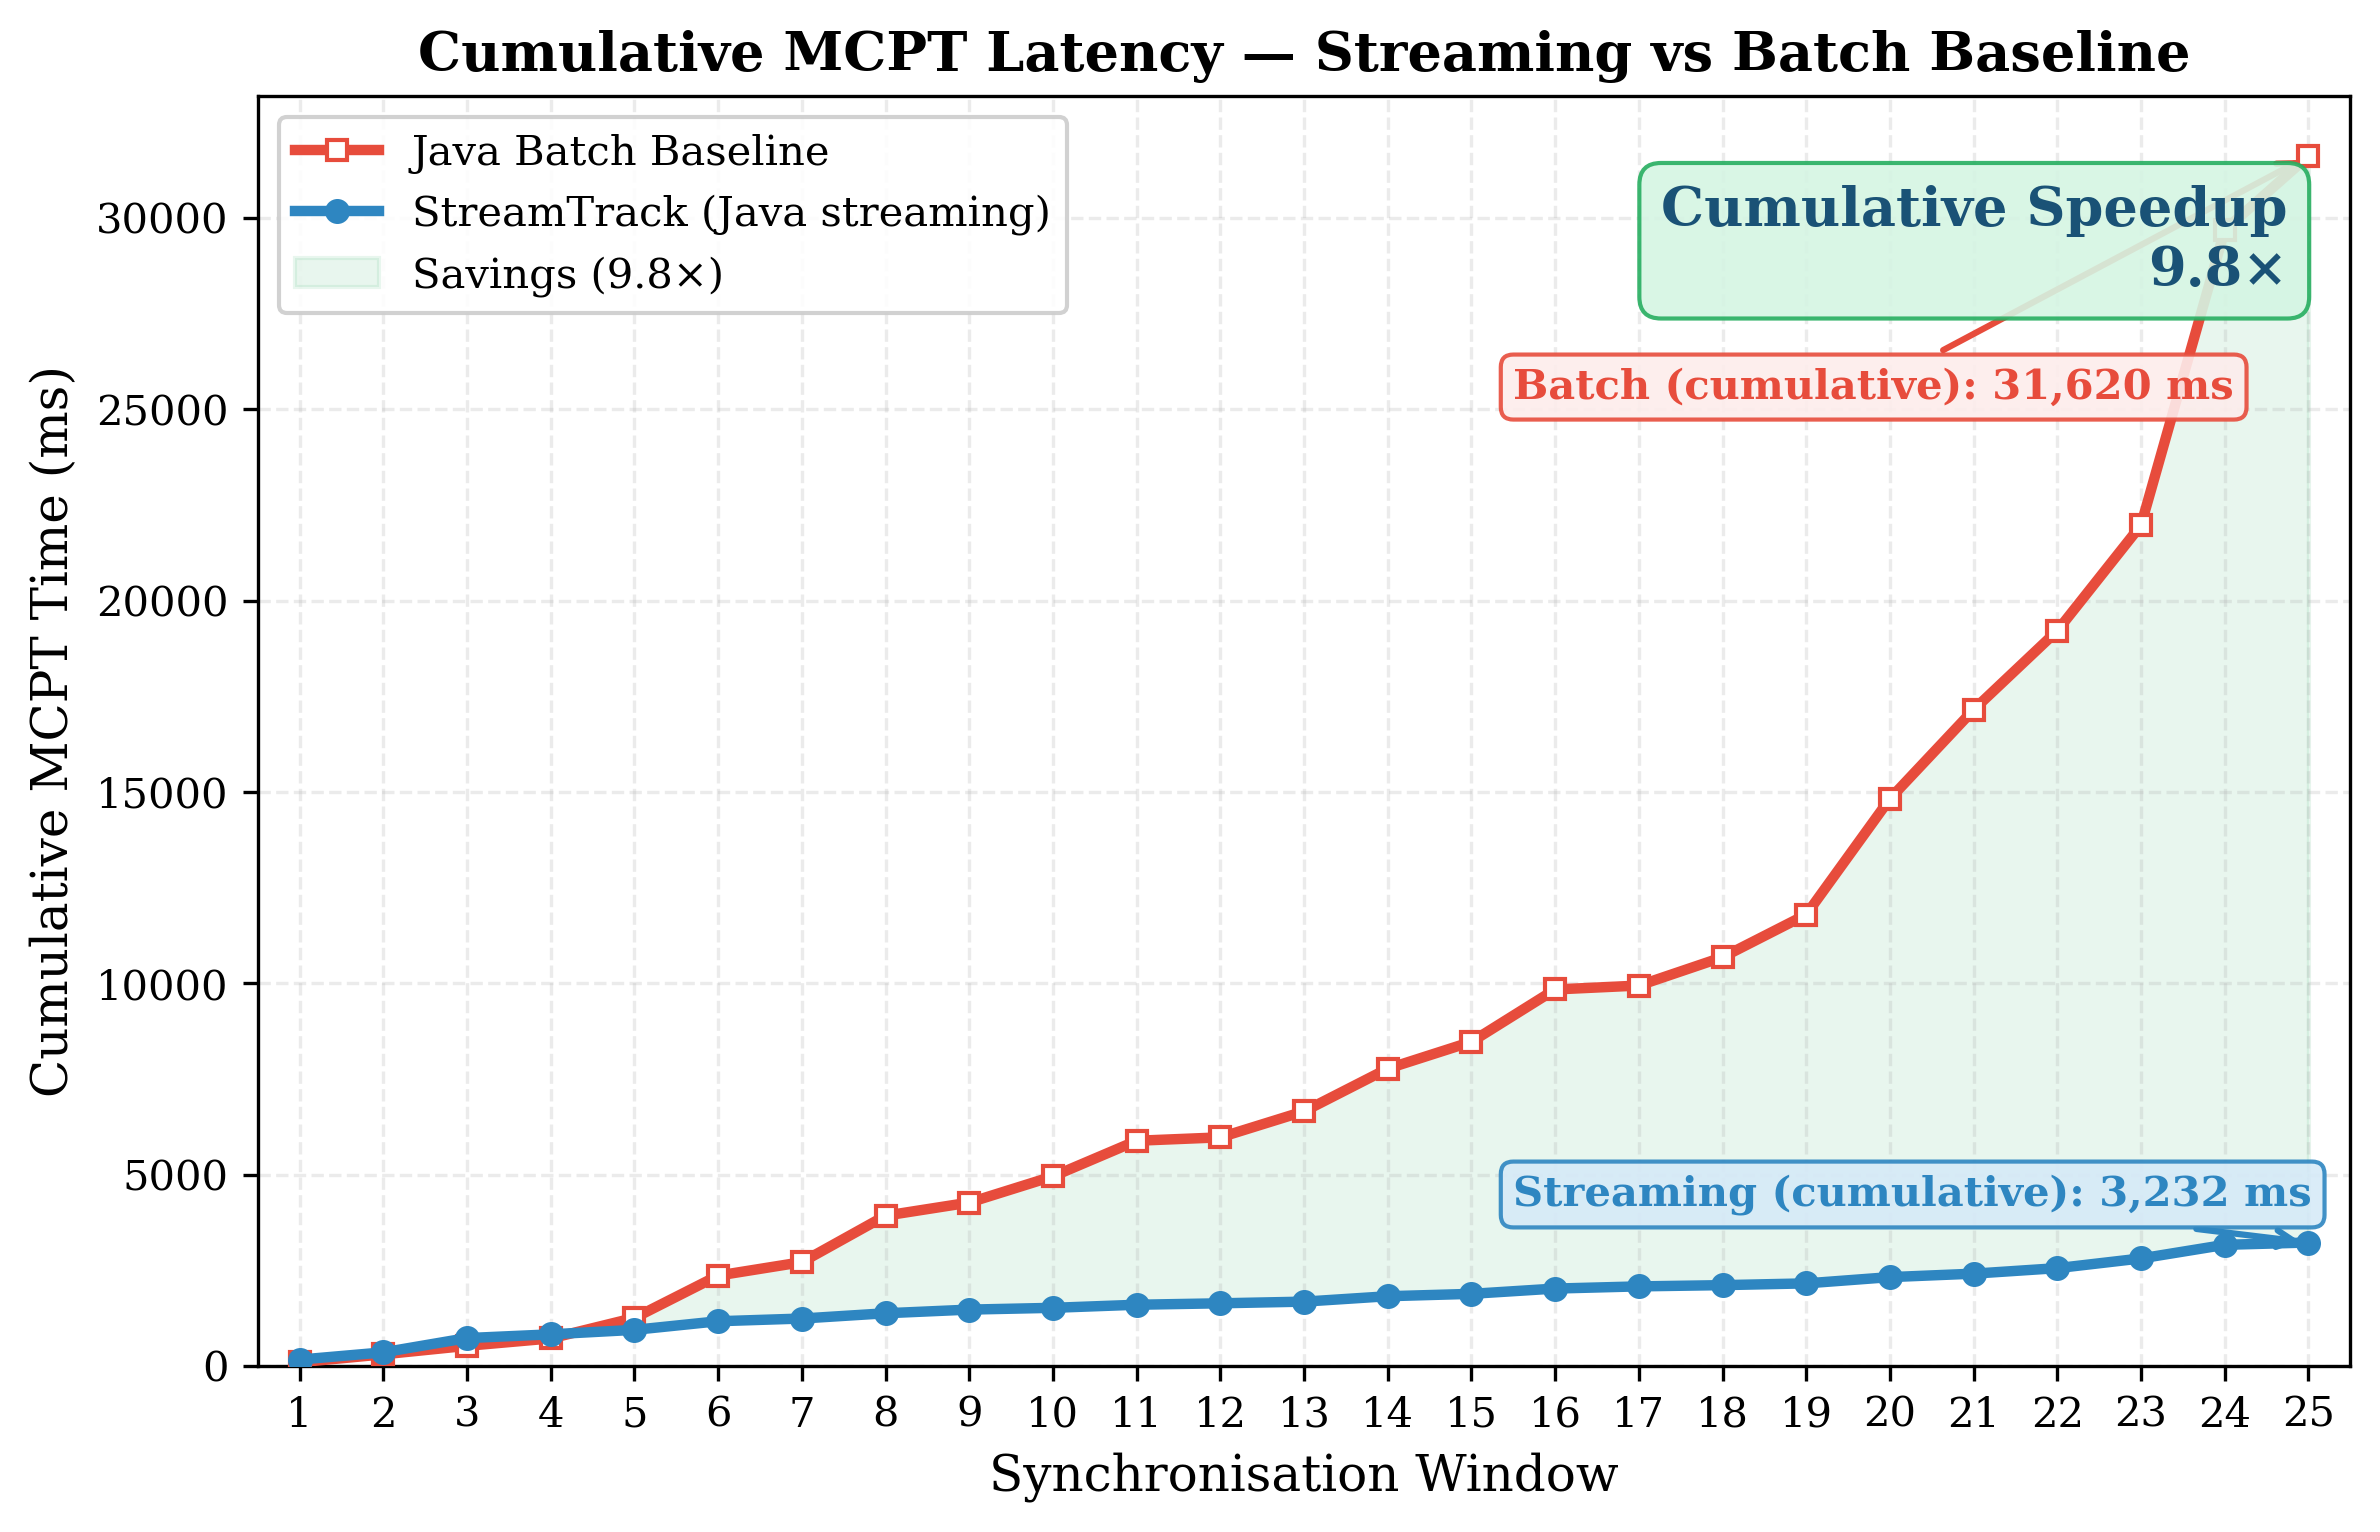
\includegraphics[width=0.9\linewidth]{Evidence/fig_cumulative_mcpt.png}
    \caption{Cumulative MCPT latency: streaming vs.\ batch baseline for the 4-camera Woven WTS dataset. The streaming pipeline processes data incrementally, accumulating to 3,232~ms over 25 windows. The batch curve is constructed from real per-window measurements: at each window $n$, the pipeline re-loads and re-processes all accumulated data from scratch, yielding a total of 31,620~ms for 25 windows. The architectural speedup reaches \textbf{9.8$\times$}.}
    \label{fig:cumulative_mcpt}
\end{figure}

Figure~\ref{fig:cumulative_mcpt} visualises the cumulative latency divergence. The streaming architecture accumulates MCPT time gradually, reaching 3,232 ms across all 25 windows because each window processes only newly arriving data. The batch baseline, by contrast, re-processes the full accumulated state from scratch at every window, producing a quadratically growing cost curve that culminates in 31,620~ms. The cumulative speedup of \textbf{9.8$\times$} confirms that the streaming architecture neutralises the scalability bottleneck that plagues conventional batch-oriented MCPT implementations.

These results validate the central thesis of this work: the scalability limitations of MCOT are architectural rather than algorithmic. By re-architecting the pipeline around streams and tables, where state lives incrementally in relational tables and per-window processing is proportional to newly arriving data, the system sustains real-time throughput even as accumulated state grows, without sacrificing tracking fidelity. 

By defining association as a join over a reconfigurable \texttt{CameraTopologyTable}, the search space no longer grows with the global camera count but with the size of each topological cluster. While our largest experiment uses nine cameras, the $\binom{m}{2} \to \sum \binom{n_i}{2}$ reduction means the per-group load remains bounded as the global network grows, making deployments beyond the scale demonstrated here a plausible projection from this foundation. The bottleneck in our system has shifted from algorithmic complexity to local streaming I/O, yielding a predictable processing cost that scales with cluster size rather than the total camera count.

Because both the batch baseline and the streaming implementation share the same JVM, math library (ND4J/OpenBLAS), and heap configuration, these gains are purely architectural---they derive from the streams-and-tables design rather than from language-level performance differences. Overall, the system processes a 4-camera window in approximately 129~ms on average (streaming) vs.~1,265~ms (batch per-window average), demonstrating robust capability for real-time operation in diverse multi-camera environments.

\section{Discussion}\label{sec:discussion}

Expressing MCOT as continuous queries over relational state yields operational benefits beyond
raw performance. The system's state is \emph{inspectable}: developers can query the
\texttt{GlobalIDTable} at runtime using standard SQL to audit association decisions and trace
identity assignments, something impossible when identity state lives in program variables. The
operator graph is \emph{modular}: new vision operators (e.g., pose estimation) can be
integrated by adding join predicates at the engine--kernel boundary without modifying the core
architecture, and the clustering kernel itself is swappable
(Section~\ref{sec:overview:realisation}). And the deployment is \emph{reconfigurable}: both
the camera topology and the algorithmic parameters are updated by streaming events, with no
restart and no loss of accumulated state (Section~\ref{sec:eval:reconfig}).

The architecture also suggests a natural edge-to-cloud partitioning. The single-camera
tracking stage operates independently per camera and emits compact
\texttt{SingleCameraResult} events, so it can run at the edge, while the topology-aware
aggregation and global clustering are centralised in the CEP engine. Our measurements support
the feasibility of this split: the association-clustering stage processes a 4-camera window in
approximately 129~ms on average (streaming) versus 1{,}265~ms (batch per-window average) on
the Woven WTS dataset, and a topology-aware group averages $10.10 \pm 11.11$~ms per call
($9.15 \pm 8.27$~ms excluding JIT warm-up; Table~\ref{tab:9camera_performance}), indicating
that even modest centralised compute can absorb the association workload. Such a partitioning
would reduce backhaul bandwidth from raw video to lightweight feature events while preserving
a global view of identities; validating it across a real network boundary remains future
work.

Certain limitations remain. Extremely crowded scenes can produce similarity ambiguities that
topological gating cannot resolve, since gating restricts \emph{where} matches are considered
but not \emph{how} ambiguous appearances are disambiguated. Rapid lighting changes or
occlusions can cause embedding drift, which would require online adaptation of the appearance
models---an algorithmic concern deliberately outside the scope of this architectural work.
Finally, our evaluation is single-node by design (to isolate architectural effects and to
model edge-class resource constraints); measuring the architecture across a physically
distributed edge--cloud deployment is a natural next step.




\section{Conclusion and Future Work}\label{sec:conclusion}
We presented \textbf{STREAMTRACK}, a relational streams-and-tables architecture for multi-camera object tracking. By recasting MCOT as a continuous query problem and utilizing topology-aware stream joins, we achieved a \textbf{9.8$\times$ overall speedup} over an equivalent JVM batch baseline on the Woven WTS dataset, with up to \textbf{300$\times$} speedup in the representative selection stage and \textbf{236$\times$} in clustering. Because both the batch and streaming implementations share the same language, runtime, and math library, these gains are purely architectural---they validate the central claim that MCOT scalability is an architectural, not algorithmic, problem. Scaling the NVIDIA SmartSpaces network with topology-aware partitioning yields a further \textbf{4.16$\times$} (up to \textbf{4.27$\times$} in steady state excluding JVM warm-up) latency reduction per association call. Our system ensures real-time performance even as the camera network grows, while providing an architecture that supports unique operational benefits like runtime reconfigurability and SQL-based inspectability.

% TODO[Student]: if SmartSpaces parity lands per the TODO above, extend the conclusion's
% parity sentence accordingly.

\paragraph{Future work.}
Future directions include: (i) multi-hop topology reasoning, where cameras beyond immediate neighbors contribute to association via transitive similarity; and (ii) learning topology weights from historical data to dynamically adjust join selectivity.

% \bibliographystyle{plain}
\bibliographystyle{elsarticle-num}
\bibliography{references}

\end{document}
